%*****************************************************************************************
%*********************************** Second Chapter **************************************
%*****************************************************************************************


%\newcommand\mycmd[2][]{%
%  \ifstrempty{#1}{%
    % something with #2
%  }{%
    % some other thing with #1 and #2
%  }%
%}

\newcommand{\discrete}[1]{\widehat{#1}}
\newcommand{\apprx}[1]{\widetilde{#1}}
\newcommand{\normed}[1]{\overline{#1}}


\newcommand{\thetaA}{\delta\theta}


\newcommand\R[1][]{
  \ifstrempty{#1}{
    \mathbf{R}
  }{
    \mathbf{R}\left( #1 \right)
  }
} 

% The scaling for the matrix
\newcommand\Scale[1][]{
  \ifstrempty{#1}{
    \vec{S}
  }{
    \vec{S}\left( #1 \right)
  }
} 

% ----- qR definitions -------
% The scaling for the matrix
\newcommand\qS[1][]{
  \ifstrempty{#1}{
    \vec{qS}
  }{
    \vec{qS}\left( #1 \right)
  }
} 

% The matrix
\newcommand\qR[1][]{
  \ifstrempty{#1}{
    \mathbf{qR}
  }{
    \mathbf{qR}\left( #1 \right)
  }
} 


% The matrix in the 0 < theta < Pi/6 region \dfR[\theta]=\fRO[ \dfRe[\theta], \theta]
\newcommand\qRe[1][]{
  \ifstrempty{#1}{
     \mathbf{qR}\text{e}
  }{
     \mathbf{qR}\text{e}\left( #1 \right)
  }
} 

% The perturbation to the matrix 
\newcommand\dqR[1][]{
  \ifstrempty{#1}{
    \delta \mathbf{qR}
  }{
    \delta \mathbf{qR}\left( #1 \right)
  }
} 

% The perturbation to the matrix in the 0 < theta < Pi/6 region \dqR[\theta]=\fRO[ \dqRe[\theta], \theta]
\newcommand\dqRe[1][]{
  \ifstrempty{#1}{
    \delta \mathbf{qR}\text{e}
  }{
    \delta \mathbf{qR}\text{e}\left( #1 \right)
  }
} 


% ----- fR definitions -------
% The scaling for the matrix
\newcommand\fS[1][]{
  \ifstrempty{#1}{
    \vec{fS}
  }{
    \vec{fS}\left( #1 \right)
  }
} 
% The sign for the scaling for the matrix
\newcommand\fSs[1][]{
  \ifstrempty{#1}{
    \vec{fSs}
  }{
    \vec{fSs}\left( #1 \right)
  }
} 

% The scaling ordering for the matrix
\newcommand\fSO[1][]{
  \ifstrempty{#1}{
    \text{fSO}
  }{
    \text{fSO}\left[ #1 \right]
  }
} 

% The scaling for the matrix  in the 0 < theta < Pi/6 region
\newcommand\fSe[1][]{
  \ifstrempty{#1}{
    \text{fSe}
  }{
    \text{fSe}\left[#1 \right)
  }
} 

% The matrix
\newcommand\fR[1][]{
  \ifstrempty{#1}{
    \mathbf{fR}
  }{
    \mathbf{fR}\left( #1 \right)
  }
} 

% The matrix in the 0 < theta < Pi/6 region \dfR[\theta]=\fRO[ \dfRe[\theta], \theta]
\newcommand\fRe[1][]{
  \ifstrempty{#1}{
     \mathbf{fR}\text{e}
  }{
     \mathbf{fR}\text{e}\left( #1 \right)
  }
} 

% The matrix in the 0 < theta < Pi/6 region \dfR[\theta]=\fRO[ \dfRe[\theta], \theta]
\newcommand\fRm[1][]{
  \ifstrempty{#1}{
     \mathbf{fR}\text{m}
  }{
     \mathbf{fR}\text{m}\left( #1 \right)
  }
} 

% The perturbation to the matrix 
\newcommand\dfR[1][]{
  \ifstrempty{#1}{
    \delta \mathbf{fR}
  }{
    \delta \mathbf{fR}\left( #1 \right)
  }
} 

% The perturbation to the matrix in the 0 < theta < Pi/6 region \dfR[\theta]=\fRO[ \dfRe[\theta], \theta]
\newcommand\dfRe[1][]{
  \ifstrempty{#1}{
    \delta \mathbf{fR}\text{e}
  }{
    \delta \mathbf{fR}\text{e}\left( #1 \right)
  }
} 

% The Ordering function which puts fRe into the correct form for the other regions \fR[\theta]=\fRO[ \fRe[\theta], \theta]
\newcommand\fRO[1][]{
  \ifstrempty{#1}{
    \mathbf{fR}\text{O}
  }{
    \mathbf{fR}\text{O}\left[#1\right]
  }
}

% The Ordering function which puts fRe into the correct form for the other regions \fR[\theta]=\fRO[ \fRe[\theta], \theta]
\newcommand\fROm[1][]{
  \ifstrempty{#1}{
    \widehat{\mathbf{fR}\text{O}}
  }{
    \widehat{\mathbf{fR}\text{O}}\left[#1\right]
  }
}

% --------- rR

\newcommand\rR[1][]{
  \ifstrempty{#1}{
    \mathbf{rR}
  }{
    \mathbf{rR}\left( #1 \right)
  }
} 

\newcommand\nR[1][]{
  \ifstrempty{#1}{
    \normed{\mathbf{R}}
  }{
    \normed{\mathbf{R}}\left( #1 \right)
  }
} 

\newcommand\nRa[1][]{
  \ifstrempty{#1}{
    \apprx{\normed{\mathbf{R}}}
  }{
   \apprx{ \normed{\mathbf{R}}} \left( #1 \right)
  }
} 

\newcommand\dnR[1][]{
  \ifstrempty{#1}{
    \normed{\delta\mathbf{R}}
  }{
   \normed{\delta\mathbf{R}} \left( #1 \right)
  }
} 


% The scaling for the matrix
\newcommand\rS[1][]{
  \ifstrempty{#1}{
    \vec{rS}
  }{
    \vec{rS}\left( #1 \right)
  }
} 


% ----- nR definitions -------
% The scaling for the matrix
\newcommand\nS[1][]{
  \ifstrempty{#1}{
    \vec{nS}
  }{
    \vec{nS}\left( #1 \right)
  }
} 

\newcommand{\um}{\scalebox{0.75}[1.0]{\( - \)}}
\newcommand{\Pii}[1]{\frac{\pi}{#1} }
\newcommand{\sine}[1]{\sin \left( \scalebox{0.75}[1.0]{\( #1 \)}\right)}
\newcommand{\cosine}[1]{\cos \left( \scalebox{0.75}[1.0]{\( #1 \)} \right)}
\newcommand{\secant}[1]{\sec \left( \scalebox{0.75}[1.0]{\( #1 \)}\right)}
\newcommand{\cosecant}[1]{\csc \left( \scalebox{0.75}[1.0]{\( #1 \)}\right)}

% \newcommand{\fRe}[1]{\mathbf{fR}\text{e}\left(#1\right) }

% \newcommand{\dfRe}[1]{\delta \mathbf{fR}\text{e}\left(#1\right) }

% \newcommand{\fRO}[1]{\mathbf{fR}\text{O}\left[#1\right] }

\newcommand{\fReq}[1]{\text{fRe}\left( \scalebox{0.75}[1.0]{\( #1 \)}\right) }

\newcommand{\unitDst}{\text{uDst}} % Destination in the unit range 0:1
\newcommand{\uDst}{\unitDst}       % Destination in the unit range 0:1
\newcommand{\intDst}{\text{iDst}}  % Destination in the integer range dstMin:dstMax
\newcommand{\iDst}{\intDst}        % Destination in the integer range dstMin:dstMax
\newcommand{\dstMax}{\text{dstMax}}      % Destination integer range maximum
\newcommand{\dstMin}{\text{dstMin}}      % Destination integer range mimimum
\newcommand{\dstRange}{\text{dstRange}}  % Destination integer range
\newcommand{\discreteDst}{\widetilde{\uDst}}   % Destination found using the discretized transformation matrix
\newcommand{\dDst}{\discreteDst}               % Destination found using the discretized transformation matrix
\newcommand{\delDst}{\delta\uDst}              % Error in the Destination found using the discretized transformation matrix

\newcommand{\unitT}{\text{uT}}             % Rotated values in the unit range 0:1
\newcommand{\uT}{\unitT}                   % Rotated values in the unit range 0:1
\newcommand{\intT}{\text{iT}}              % Rotated values in the integer range tMin:tMax
\newcommand{\iT}{\intT}                    % Rotated values in the integer range tMin:tMax
\newcommand{\tMax}{\text{tMax}}            % Rotated values integer range maximum
\newcommand{\tMin}{\text{tMin}}            % Rotated values integer range mimimum
\newcommand{\tRange}{\text{tRange}}        % Rotated values integer range
\newcommand{\discreteT}{\widetilde{\uT}}   % Rotated values found using the discretized transformation matrix
\newcommand{\dT}{\discreteT}               % Rotated values found using the discretized transformation matrix
\newcommand{\delT}{\delta\uT}              % Error in the Rotated values found using the discretized transformation matrix

\newcommand{\unitSrc}{\text{uSrc}}       % Source in the unit range 0:1
\newcommand{\uSrc}{\unitSrc}             % Source in the unit range 0:1
\newcommand{\intSrc}{\text{iSrc}}        % Source in the integer range srcMin:srcMax
\newcommand{\iSrc}{\intSrc}              % Source in the integer range srcMin:srcMax
\newcommand{\srcMax}{\text{srcMax}}      % Source integer range maximum
\newcommand{\srcMin}{\text{srcMin}}      % Source integer range mimimum
\newcommand{\srcRange}{\text{srcRange}}  % Source integer range

\newcommand{\unitX}{\text{uX}}       % Source in the unit range 0:1
\newcommand{\uX}{\unitX}             % Source in the unit range 0:1
\newcommand{\intX}{\text{iX}}        % Source in the integer range xMin:xMax
\newcommand{\iX}{\intX}              % Source in the integer range xMin:xMax
\newcommand{\xMax}{\text{xMax}}      % Source integer range maximum
\newcommand{\xMin}{\text{xMin}}      % Source integer range mimimum
\newcommand{\xRange}{\text{xRange}}  % Source integer range

\newcommand{\unitY}{\text{uY}}       % Destination in the unit range 0:1
\newcommand{\uY}{\unitY}             % Destination in the unit range 0:1
\newcommand{\intY}{\text{iY}}        % Destination in the integer range yMin:yMax
\newcommand{\iY}{\intY}              % Destination in the integer range yMin:yMax
\newcommand{\yMax}{\text{yMax}}      % Destination integer range maximum
\newcommand{\yMin}{\text{yMin}}      % Destination integer range mimimum
\newcommand{\yRange}{\text{yRange}}  % Destination integer range

\newcommand{\unitR}{\text{uR}}
\newcommand{\uR}{\unitR}
\newcommand{\intR}{\text{iR}}
\newcommand{\iR}{\intR}
\newcommand{\discreteR}{\widetilde{\uR}}
\newcommand{\dR}{\discreteR}
\newcommand{\delR}{\delta\uR}
\newcommand{\rRange}{\text{rRange}}  % the discretization of the rotation matrix


\chapter{Color Spaces and Information Storage for Computer Vision Processing} \label{sec:Chap2}

\epstopdfsetup{outdir=Chapter2/Figs/PDF/}
\ifpdf
    \graphicspath{{Chapter2/Figs/Raster/}{Chapter2/Figs/PDF/}{Chapter2/Figs/}}
\else
    \graphicspath{{Chapter2/Figs/Vector/}{Chapter2/Figs/}}
\fi


\section{Constructing a New Color Space}\label{sec:ConstructingANewColorSpace}

In order to construct a new color space, we need to consider the coordinate system of the new color space, the orientation of the new color space, and the fidelity of the discrete representation of the axes.

The first consideration is most easily decided; because there's little obvious advantage otherwise, we choose a Cartesean coordinate system as this allows for a straightforward transformation involving only rotation, translation and scaling. Because we're interested in the color information in the image, it's useful to design the color space so there is a luminosity axis. This choice determines two of three rotational degrees of freedom, as will be discussed below.

As for the discrete representation of the axes, it's desired that all the information captured pertaining to a hand should be preserved; all other information is irrelevant. However, here we'll consider only the effect of a rotation and scaling on the discrete representation.


\subsection{Camera RGB and Normalization for Discrete Range}\label{sec:CameraRGB}

Due to the iPhone hardware being locked down at the application level, we do not have access to the raw camera feed. We do, however, have access to the post-processing (color-rebalanced and white-point-corrected) 8-bit RGB image data.

Because we're searching for particular points in the real color space --- which, being a continuous function, is infinite dimensional --- there is a possibility in the future that larger multi-channel color spaces will be much more common, such as the 8-channel color spaces currently in development. Though most such cameras are primarily designed for post-production editing for still pictures and film (e.g. changing the lighting independent of the scene), as well as visual effects, the possibilities for computer vision are exciting. However, computer vision tasks are computationally intensive, and more often than not require operation in real time, so there is a natural inclination to shy away from large data sets in practical computer vision applications; many tasks are done in grayscale or single-channel processing to expedite the process.

As such, there is a need to develop techniques which keep the relevant information while quickly and efficiently discarding the irrelevant information. This is true for the RGB space at the moment, and the aim of this first part of the work.


\subsection{Rotation Matrix}\label{sec:RotationMatrix}
Any rotation about an axis can be represented by a 3x3 square matrix in a 3D space. Since they are invertible, they're guaranteed to be non-singular. However, as there are many ways in which to rotate an object from one position to another, or use a combination of different rotations to get to the same point, they aren't necessarily unique. For this application, we require rotation about three different axes, which can be expressed thus:


\begin{alignat}{1}
\R_x(\theta) &= \begin{bmatrix}
1 & 0 & 0 \\
0 & \cos \theta &  -\sin \theta \\[3pt]
0 & \sin \theta  &  \cos \theta \\[3pt]
\end{bmatrix} \\[6pt]
\R_y(\theta) &= \begin{bmatrix}
\cos \theta & 0 & \sin \theta \\[3pt]
0 & 1 & 0 \\[3pt]
-\sin \theta & 0 & \cos \theta \\
\end{bmatrix} \\[6pt]
\R_z(\theta) &= \begin{bmatrix}
\cos \theta &  -\sin \theta & 0 \\[3pt]
\sin \theta & \cos \theta & 0\\[3pt]
0 & 0 & 1\\
\end{bmatrix}
\end{alignat}


Any rotation which orients the RGB color space such that one of the new axes lies along the luminosity direction is sufficient; a rotation which aligns the L axis along the luminosity direction is produced by a rotation of $\frac{\pi}4$ about the red (\textbf{R}) axis, followed by a rotation of $\arctan{\frac{1}{\sqrt{2}}}$ about the green (\textbf{G}) axis. This leaves one free rotational degree of freedom about the L axis. The resulting rotation matrix is given by:

\begin{equation}
\R_{xyz}(\theta) =
\begin{pmatrix}
 \frac{1}{\sqrt{3}} & \frac{1}{\sqrt{3}} & \frac{1}{\sqrt{3}} \\
 -\sqrt{\frac{2}{3}} \sine{\theta +\Pii{6} } & \sqrt{\frac{2}{3}} \cos (\theta ) & -\sqrt{\frac{2}{3}} \sine{\Pii{6}-\theta } \\
 -\sqrt{\frac{2}{3}} \cos \left(\theta +\Pii{6}\right) & -\sqrt{\frac{2}{3}} \sin (\theta ) & \sqrt{\frac{2}{3}} \cos \left(\Pii{6}-\theta \right) \\
\end{pmatrix}
\end{equation}


Where $\theta$ is the remaining rotational degree of freedom.

Using the standard rotation matrices, we get a luminosity axis which spans the range $0:\sqrt{3}$. However, the length of the two remaining axes are dependent on the value of $\theta$ used. This is a problem because, ultimately, we want the axes to fit in a range of an appropriate data type. It would be more useful to have a matrix which provided the specified rotation and scaled the axis to known lengths. In the case of the luminosity, this is straightforward; simply divide by $\sqrt{3}$. In the case of the other two axes, we need an explicit form for the lengths of the axis resulting from the rotation.

Because the absolute values of the axes in the color space have no meaning, we're only interested in the position along the axis relative to its start and end, equivalent to talking about the position in the axis relative to $0:1$, compared to about $0:255$ in unsigned, 8-bit integers. The upside is that if we're rotating the cube about its corner, we're interested in the minimum and maximum values possible along the new axis direction, which will correspond to a corner of the RGB cube. With the L axis aligned along the luminosity direction, the range of the L axis is 0 to $\sqrt{3}$. The x and y axes are symmetrical, spanning a range centered on 0. The range of their values is dependent upon the remaining degree of freedom.

We need to know, in each of the axes, how far out each point is. Because we're effectively rotating a hexagon, whatever the answer is, we know the function is going to be periodic, repeating every $\frac{\pi}{3}$ radians, so we only have to solve it in the $0:\frac{\pi}{3}$ region and then generalize. First we take the coordinates of the RGB cube and perform the rotation to find the values in the new color space.


\begin{multline}\label{eq:YabCube}
  \R_{xyz}(\theta)\cdot
\begin{pmatrix}
 0 & 1 & 1 & 0 & 0 & 0 & 1 & 1 \\
 0 & 0 & 1 & 1 & 1 & 0 & 0 & 1 \\
 0 & 0 & 0 & 0 & 1 & 1 & 1 & 1 \\
\end{pmatrix}
 = \\
\resizebox{\textwidth}{!}{%
$\displaystyle
\begin{pmatrix}
 0 & \frac{1}{\sqrt{3}} & \frac{2}{\sqrt{3}} & \frac{1}{\sqrt{3}} & \frac{2}{\sqrt{3}} & \frac{1}{\sqrt{3}} & \frac{2}{\sqrt{3}} & \sqrt{3} \\
 0 & -\sqrt{\frac{2}{3}} \sin \left(\theta +\Pii{6}\right) & \sqrt{\frac{2}{3}} \sin \left(\Pii{6}-\theta \right) & \sqrt{\frac{2}{3}} \cos (\theta ) & \sqrt{\frac{2}{3}} \sin \left(\theta +\Pii{6}\right) & -\sqrt{\frac{2}{3}} \sin \left(\Pii{6}-\theta \right) & -\sqrt{\frac{2}{3}} \cos (\theta ) & 0 \\
 0 & -\sqrt{\frac{2}{3}} \cos \left(\theta +\Pii{6}\right) & -\sqrt{\frac{2}{3}} \cos \left(\Pii{6}-\theta \right) & -\sqrt{\frac{2}{3}} \sin (\theta ) & \sqrt{\frac{2}{3}} \cos \left(\theta +\Pii{6}\right) & \sqrt{\frac{2}{3}} \cos \left(\Pii{6}-\theta \right) & \sqrt{\frac{2}{3}} \sin (\theta ) & 0 \\
\end{pmatrix}$}
\end{multline}


The extent of the new axis is found by taking the maximum and minimum values of each row, i.e. the extreme corner positions relative to each new axis. An additional symmetry of the hexagonal projection of the RGB cube allows us to say that --- whatever functional form is taken by one of the $\theta$ dependant ranges --- the other can be found by a simple phase shift. So, recognizing that the minimum value is simply $-1$ times the maximum, we have simplified the problem to solving:

\begin{equation}\label{eq:AxisRangeMinMax}
 \max\left(\pm\frac{\sin (\theta )}{\sqrt{6}}\pm\frac{\cos (\theta )}{\sqrt{2}}, \pm\sqrt{\frac{2}{3}} \sin (\theta ) \right) \quad \text{Where} \quad 0\leq \theta \leq \frac{\pi}{3}
\end{equation}

A graphical representation of the problem can be seen in Figure~\ref{eq:YabCube}.

\begin{figure}[h!]
  \centering
    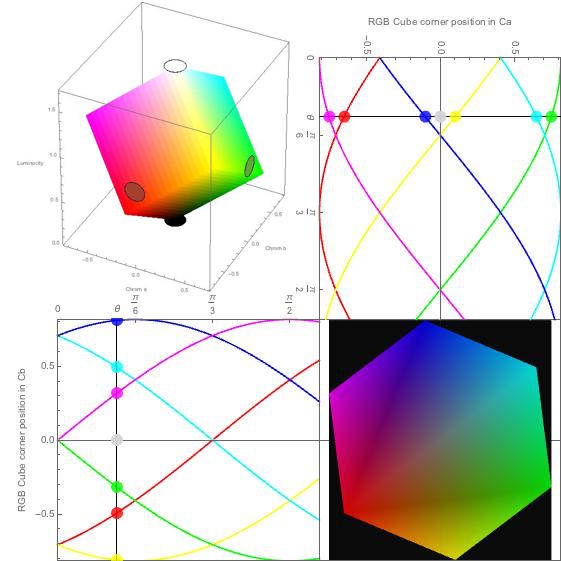
\includegraphics[width=\textwidth]{Chapter2/Figs/CornersOf_theRGBCube.jpg}
    \caption{Evaluation of the color space problem. The cube in the top-left shows the positions of the axes in the rotated space; the white and black disks on the vertical axis represent the white point and black point of the luminosity axis, and the other disks represent the ends of the chromatic axes \textbf{Ca} and \textbf{Cb}. The graphs in the top-right and bottom-left show the positions of the corners of the RGB cube relative to the chromatic axes \textbf{Ca} and \textbf{Cb}. The bottom-right graphic shows the RGB cube viewed down the luminosity axis. The graphics were generated by interactive code written in Mathematica. The value of $\theta$ was an arbitrary value from a snapshot taken from the interactive graphic.}\label{fig:YABCubeEval}
\end{figure}

In the range $0:\frac{\pi}{3}$, both sin and cos are positive, therefore the axis ranges are given by the following:

\begin{tabular}{|c|c|c|}
  \hline
  % after \\: \hline or \cline{col1-col2} \cline{col3-col4} ...
    & Min & Max \\ \hline
  L & \(0\) & \(\sqrt{3}\) \\
  Ca & \(- \sqrt{\frac{2}{3}} \cos \left(\Pii{6}-(\left(\theta -\Pii{6}\right) \bmod \frac{\pi }{3})\right) \)&\( \sqrt{\frac{2}{3}} \cos \left(\Pii{6}-(\left(\theta -\Pii{6}\right) \bmod \frac{\pi }{3})\right) \)\\
 Cb & \(-\sqrt{\frac{2}{3}} \cos \left(\Pii{6}-(\theta  \bmod \frac{\pi }{3})\right) \)&\( \sqrt{\frac{2}{3}} \cos \left(\Pii{6}-(\theta  \bmod \frac{\pi }{3})\right) \)\\
  \hline
\end{tabular}

The lengths of the axis after rotation are given by:

\begin{equation}\label{eq:L}
\mathbf{L}(\theta) =
\begin{pmatrix}
\sqrt{3} \\
 \sqrt{\frac{2}{3}} \sin \left(\widetilde{\vartheta}\right) + \sqrt{2} \cos \left(\widetilde{\vartheta}\right) \\  
\sqrt{\frac{2}{3}} \sin \left(\widetilde{\theta}\right) + \sqrt{2} \cos \left(\widetilde{\theta}\right) 
\end{pmatrix}
\quad \text{where}  \quad 
\begin{array}{c}
\widetilde{\theta} = \theta  \bmod \frac{\pi }{3} \\ 
\widetilde{\vartheta} = \left(\theta - \Pii{6}\right) \bmod \frac{\pi }{3}
\end{array}
\end{equation}

It is convenient to produce a transformation which will result in axes of known length. Because the rotation cannot include a translation, we desire a transformation matrix which will result in the ranges $0:1$, -$\frac{1}2:\frac{1}2$, and -$\frac{1}2:\frac{1}2$. Such a transformation is easily obtained by multiplying the rotation matrix by a diagonal matrix with the reciprocal of the maximums found above placed along the diagonal. This will scale each axis to a unit length.

The normalized 'rotation' matrix is given by:


\begin{align}\label{eq:NormRxyz3}
 \overline{\R}_{xyz}(\theta) &= \nS[\theta] \otimes R_{xyz}(\theta) \\
&=\left(
\begin{array}{c}
 \frac{1}{\sqrt{3}}  \\
 \frac{1}{\sqrt{\frac{2}{3}} \sin \left(\widetilde{\vartheta}\right) + \sqrt{2} \cos \left(\widetilde{\vartheta}\right)} \\
 \frac{1}{\sqrt{\frac{2}{3}} \sin \left(\widetilde{\theta}\right) + \sqrt{2} \cos \left(\widetilde{\theta}\right)  }  \\
\end{array}
\right)
\bigotimes
R_{xyz}(\theta)
\end{align}

This matrix is no longer technically a rotation matrix as its inverse is no longer equal to its transpose. It now equal to:

\begin{equation}\label{eq:NormRxyz3Inverse}
 \overline{\R}_{xyz}^{-1}(\theta) =
 R_{xyz}(\theta)^{T} \bigotimes
\left(
\begin{array}{ccc}
 \frac{1}{\sqrt{3}}  &
 \frac{1}{L_2(\theta)} &
 \frac{1}{L_3(\theta) }
\end{array}
\right)
\end{equation}

\subsection{Representing the Rotation}

The final piece of the metaphorical jigsaw is to add the capability to deal with the machine handling of the numerics. The transforms as defined above assume the capacity to represent the resulting numbers. Unfortunately, on a device, the numerics are not handled in such a pure way and --- whilst we are uninterested in the information overflow outside the destination representation --- this can cause instabilities in a practical implementation. In the development of the algorithm, it is therefore necessary to define these bounds. In the unit space, these bounds have already been defined by Equation~\ref{eq:L}; so long as the axis length can be represented on the device between these bounds, then overflow and underflow can be dealt with using a simple conditional statement.

It is significantly advantageous to perform calculations using integer types, particularly given that the input and output types are integers with small ranges, meaning it's possible to construct algorithms which avoid conversion to floating point operations. To this end, we wish to determine the most efficient internal representation for the transformation.

\subsubsection{Principles of Optimization}

During the color space conversion, the pixel values are represented in three different ways: input, working and output representations. At each stage, we are concerned with preserving the information from the previous stage required by the next. For this reason, we have defined terms for the mathematical analysis of the problem, as well as terms for the algorithm development. The terms associated with each stage are as follows:

\begin{tabular}{|c|c|c|c|}
  \hline
     Data Types & Src Pixel Values & Trans Pixel Values & Dst Pixel Values \\ \hline
  What? & Input & Working & Output \\ \hline
  Where? & Initial & After Rotation & After Re-Distribution \\ \hline
  Unit Range Value & $ \uSrc $ & $\uT$ & $\uDst$ \\ \cline{1-1}
  Int Range Value & $\iSrc$ & $\iT$ & $\iDst$ \\ \cline{1-1}
  Max & $\srcMax$ & $\tMax$ & $\dstMax$ \\ \cline{1-1}
  Min & $\srcMin$ & $\tMin$ & $\dstMin$ \\ \cline{1-1}
  Range & $\srcRange$ & $\tRange$ & $\dstRange$ \\
  \hline
\end{tabular}

The rotation operation consists of 9 multiplications and 6 additions and constitutes the majority of the computational cost. It is this operation which we will focus our optimization efforts upon. The redistribution transformation, which comes after the rotation, processes each pixel channel value separately. This allows us to pull apart the rotation matrix by scaling each row arbitrarily, handing the knowledge of the scaling to the distribution. The goal of this section is to represent the matrix multiplication in such a way that we avoid floating-point operations.

\begin{equation}\label{eq:NormRxyz4}
 \R[\theta] =
\left(
\begin{array}{c}
 -  \\
 \text{Scale} \\
 -  \\
\end{array}
\right)
\bigotimes
\qR[\theta]\;\text{where}\quad{\qR[\theta]\in\mathbb{Z}}
\end{equation}

Given an infinite set of integers, this is not a problem. However, we wish to choose $\qR$ to lie in a finite range, which depends on the color depth of the source. Ideally, we'd like the result of the rotation to have a bit depth not greater than twice the bit depth of the source, i.e. for 8-bit pixel values, we would like the rotated LCaCb values to be expressible as 16-bit integers. To accommodate 3 multiplications and 2 additions, the matrix $\qR$ needs to be represented in two fewer bits than the source.

This unit range is discretized into steps of $\frac{1}{\srcRange}$ and $\frac{1}{\tRange}$. The question then is to what degree of accuracy do we need to represent the internal numerics? If we represent the transformation in a discrete type $\discreteR$, we can express the problem in terms of the largest perturbation which can be made to the transformation without affecting the result.


\begin{equation}\label{eq:lxyPixel}
\begin{aligned}
\uR  \cdot \uSrc &= \uT  &\text{let} \quad \uR &= \dR + \delR \\
(\discreteR + \delR)  \cdot \uSrc &= \discreteT + \delT \\
\text{therefore if } \discreteR \cdot \uSrc &= \discreteT & \text{then}\quad \delR  \cdot \uSrc = \delT
\end{aligned} 
\end{equation}

The continuous rotation $\uR$ can be expressed as the sum of its discrete representation $\dR$ with a discretization factor $\rRange$ and the correction $\delR$. The elements of the discrete rotation can be expressed as rational fractions.

\begin{eqnarray}\label{eq:dRRange}
\discreteR = \dfrac{int(\uR \cdot \rRange)}{\rRange}\quad where\quad int(1.5) = 1, int (-1.5) = -1\\
therefore\quad \dfrac{-1}{\rRange} < \delR  < \dfrac{1}{\rRange}
\end{eqnarray}

It should be noted that --- unlike the source type \uSrc --- the perturbation can be negative. The definition of the function $int$ results in the sign of the perturbation matching the sign of the discretized transformation matrix. We must therefore consider both the maximum and minimum of $\delT$. As $0 \le\uSrc \le 1$ the extrema of $\delT$ are found where $\uSrc$ is a vector with elements of 0 and 1. If the matrix is decomposed into a sum of positive and negative elements $\delT = \delT_+ + \delT_-$ then the extrema are given by $\max(\delT_+ \cdot \mathbf{1})$ and $\min(\delT_- \cdot \mathbf{1})$. Where the elements are positive or negative is determined by the sign of the elements in the rotation matrix $\uR$.

\subsubsection{Factoring the Rotation}

If we were to scale the entire matrix evenly, the top row would dominate as it is always positive, and the necessary discrete representation would be characterised by $\rRange = 3 \; \tRange$. This would, however, necessitate the matrix being stored in a data type with at least 2 more bits than the source type.

The second and third rows each sum to zero ($\uR \cdot \mathbf{1} = [\sqrt{3},0,0]$, where $\mathbf{1}$ is a vector of ones), allowing us to state that each of the rows has one element of the opposite sign to the other two elements. The discretization for the second and third rows then only requires $\rRange = 2 \; \tRange$. It is also possible to pull out common factors from the rows, resulting in all elements taking values between -1 and 1.

\begin{equation}
\uR(\theta) =
\left(
\begin{array}{c}
 \frac{1}{\sqrt{3}} \\
 \sqrt{\frac{2}{3}}  \\
 \sqrt{\frac{2}{3}} \\
\end{array}
\right) \bigotimes
\begin{pmatrix}
 1 & 1 & 1 \\
 -\sin \left(\theta +\Pii{6}\right) &  \cos (\theta ) &  \sin \left(\theta -\Pii{6}\right) \\
 -\cos \left(\theta +\Pii{6}\right) & - \sin (\theta ) & \cos \left(\theta -\Pii{6}\right) \\
\end{pmatrix}
\end{equation}

To facilitate the quantization, we next factor the second and third rows such that the largest element of each row equals exactly 1. As previously mentioned, the largest element has the opposite sign to the other two elements in a given row. So, the steps required to perform the factorization are as follows:

\begin{itemize}
\item{Find the sign of each of the elements.}
\item{Determine which of those elements is of the opposite sign.}
\item{Factor each row by that largest element.}
\end{itemize}

The sign of the elements is most easily seen by looking at the rotation as phase shifted sine functions.
\begin{equation}
\rR[\theta]=
\begin{pmatrix}
 1 & 1 & 1 \\
 \sine{\theta -\frac{5 \pi }{6}}  & \sine{\theta +\frac{3 \pi }{6}}  & \sine{\theta -\Pii{6}}  \\
 \sine{\theta -\frac{2 \pi }{6}}  & \sine{\theta -\frac{6 \pi }{6}}  & \sine{\theta +\frac{2 \pi }{6}}  \\
\end{pmatrix}
\end{equation}

So the signs look like

\begin{equation}
\begin{pmatrix}
 1 & 1 & 1 \\
\raisebox{-10mm}{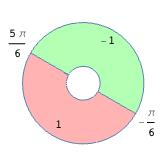
\includegraphics[width = 20mm]{Chapter2/Figs/SignOfrR21.jpg}}
\scalebox{0.68}[0.9]{\(
\begin{cases}
 1 & \frac{5 \pi }{6}\leq \theta <\frac{11 \pi }{6} \\
 \um 1 & \um \Pii{6}\leq \theta <\frac{5 \pi }{6} \\
\end{cases}
\)}
 & 
 \raisebox{-10mm}{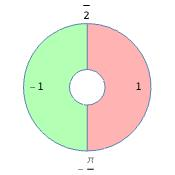
\includegraphics[width = 20mm]{Chapter2/Figs/SignOfrR22.jpg}}
 \scalebox{0.68}[0.9]{\(
\begin{cases}
 1 & \um \frac{\pi }{2}\leq \theta <\frac{\pi }{2} \\
 \um 1 & \frac{\pi }{2}\leq \theta <\frac{3 \pi }{2} \\
  \end{cases}
  \)}
 & 
 \raisebox{-10mm}{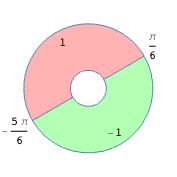
\includegraphics[width = 20mm]{Chapter2/Figs/SignOfrR23.jpg}}
 \scalebox{0.68}[0.9]{\(
\begin{cases}
 1 & \Pii{6}\leq \theta <\frac{7 \pi }{6} \\
 \um 1 & \um \frac{5 \pi}{6} \leq \theta <\Pii{6} \\
\end{cases}
\)}
 \\
 \raisebox{-10mm}{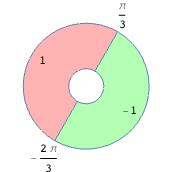
\includegraphics[width = 20mm]{Chapter2/Figs/SignOfrR31.jpg}}
 \scalebox{0.68}[0.9]{\(
\begin{cases}
 1 & \frac{\pi }{3}\leq \theta <\frac{4 \pi }{3} \\
 \um 1 & \um \frac{2 \pi }{3} \leq \theta <\frac{\pi }{3} \\
\end{cases}
\)}
 & 
\raisebox{-10mm}{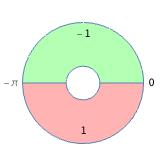
\includegraphics[width = 20mm]{Chapter2/Figs/SignOfrR32.jpg}}
\scalebox{0.68}[0.9]{\(
\begin{cases}
 1 & -\pi \leq \theta <0 \\
 -1 & 0\leq \theta <\pi  \\
 \end{cases}
 \)}
 & 
  \raisebox{-10mm}{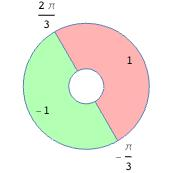
\includegraphics[width = 20mm]{Chapter2/Figs/SignOfrR33.jpg}}
  \scalebox{0.68}[0.9]{\(
\begin{cases}
 1 & \um \frac{\pi }{3}\leq \theta <\frac{2 \pi }{3} \\
 -1 & \frac{2 \pi }{3}\leq \theta <\frac{5 \pi }{3} \\
\end{cases}
\)}
 \\
\end{pmatrix}
\end{equation}

Each row is a series of three sin waves each $\frac{2\pi}{3}$ out of phase with each other. The rows are$\frac{\pi}{2}$ out of phase with each other.
The largest element changes every $\frac{\pi}{6}$ radians repeating every $\pi$ radians.

\begin{tabular}{|c|c|c|}
\hline \rule[-2ex]{0pt}{5.5ex} 
& 
\begin{tabular}{c} 
Scale : $fS[\theta]$ \\
\raisebox{-13mm}{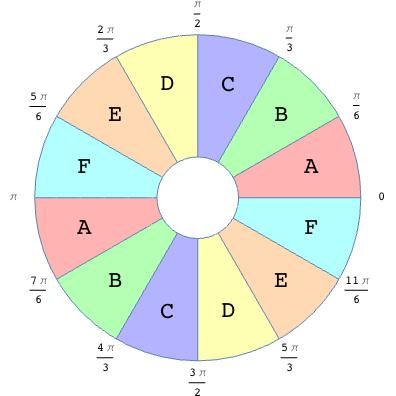
\includegraphics[width = 26mm]{Chapter2/Figs/fRWheel.jpg}} \\
\end{tabular}
&  Factored Rotation : $fR[\theta]$ \\ 
\hline \rule[-2ex]{0pt}{5.5ex} 
\bf{A} & \( \left(\!\!\!
\begin{array}{c}
 1 \\
 \cos (\theta ) \\
 \cosine{\Pii{6}-\theta } \\
\end{array}
\!\!\!\right) \)& \(  \left(\!\!\!
\begin{smallmatrix}
 1 & 1 & 1 \\
 \um\sec (\theta ) \sine{\theta +\Pii{6}} & 1 & \sec (\theta ) \sine{\theta-\Pii{6} } \\
 \um\cosine{\theta +\Pii{6}} \secant{\Pii{6}-\theta } & \um\secant{\Pii{6}-\theta } \sin (\theta ) & 1 \\
\end{smallmatrix}
\right) \)  \\ 
\hline \rule[-2ex]{0pt}{5.5ex} \bf{B} & \( \left(\!\!\!
\begin{array}{c}
 1 \\
 \um\sine{\theta +\Pii{6}} \\
 \cosine{\Pii{6}-\theta } \\
\end{array}
\!\!\!\right) \)  &  \(  \left(\!\!\!
\begin{smallmatrix}
 1 & 1 & 1 \\
 1 & \um\cos (\theta ) \cosecant{\theta +\Pii{6}} & \cosecant{\theta +\Pii{6}} \sine{\Pii{6}-\theta } \\
 \um\cosine{\theta +\Pii{6}} \secant{\Pii{6}-\theta } & \um\secant{\Pii{6}-\theta } \sin (\theta ) & 1 \\
\end{smallmatrix}
\!\!\!\right)  \) \\ 
\hline \rule[-2ex]{0pt}{5.5ex} \bf{C} & \(  \left(\!\!\!
\begin{array}{c}
 1 \\
 \um\sine{\theta +\Pii{6}} \\
 \um\sin (\theta ) \\
\end{array}
\!\!\!\right) \)  & \(  \left(\!\!\!
\begin{smallmatrix}
 1 & 1 & 1 \\
 1 & \um\cos (\theta ) \cosecant{\theta +\Pii{6}} & \cosecant{\theta +\Pii{6}} \sine{\Pii{6}-\theta } \\
 \cosine{\theta +\Pii{6}} \csc (\theta ) & 1 & \um\cosine{\Pii{6}-\theta } \csc (\theta ) \\
\end{smallmatrix}
\!\!\!\right) \)  \\ 
\hline \rule[-2ex]{0pt}{5.5ex} \bf{D} & \( \left(\!\!\!
\begin{array}{c}
 1 \\
 \sine{\theta-\Pii{6} } \\
 \um\sin (\theta ) \\
\end{array}
\!\!\!\right) \)  & \(  \left(\!\!\!
\begin{smallmatrix}
 1 & 1 & 1 \\
 \cosecant{\Pii{6}-\theta } \sine{\theta +\Pii{6}} & \um\cos (\theta ) \cosecant{\Pii{6}-\theta } & 1 \\
 \cosine{\theta +\Pii{6}} \csc (\theta ) & 1 & -\cosine{\Pii{6}-\theta } \csc (\theta ) \\
\end{smallmatrix}
\!\!\!\right) \)  \\ 
\hline \rule[-2ex]{0pt}{5.5ex} \bf{E} & \(  \left(\!\!\!
\begin{array}{c}
 1 \\
 \sine{\theta-\Pii{6} } \\
 \um\cosine{\theta +\Pii{6}} \\
\end{array}
\!\!\!\right)\)  & \(  \left(\!\!\!
\begin{smallmatrix}
 1 & 1 & 1 \\
 \cosecant{\Pii{6}-\theta } \sine{\theta +\Pii{6}} & \um\cos (\theta ) \cosecant{\Pii{6}-\theta } & 1 \\
 1 & \secant{\theta +\Pii{6}} \sin (\theta ) & \um\cosine{\Pii{6}-\theta } \secant{\theta +\Pii{6}} \\
\end{smallmatrix}
\!\!\!\right) \)  \\ 
\hline \rule[-2ex]{0pt}{5.5ex} \bf{F} &\( 
\left(\!\!\!
\begin{array}{c}
 1 \\
 \cos (\theta ) \\
 \um\cosine{\theta +\Pii{6}} \\
\end{array}
\!\!\!\right)\)   & \( \left(\!\!\!
\begin{smallmatrix}
 1 & 1 & 1 \\
 \um\sec (\theta ) \sine{\theta +\Pii{6}} & 1 & \sec (\theta ) \sine{\theta-\Pii{6}} \\
 1 & \secant{\theta +\Pii{6}} \sin (\theta ) & \um\cosine{\Pii{6}-\theta } \secant{\theta +\Pii{6}} \\
\end{smallmatrix}
\!\!\!\right)  \)  \\ 
\hline 
\end{tabular} 

By defining $\theta$ as $\theta  = \Theta + \thetaA$ --- where $\thetaA = \theta \!\!\mod \Pii{6}$, and $\Theta$ is the starting value for the region in which $\theta$ lies --- and substituting in the function $\fRe[\phi] $:

\begin{align}
\fRe[\phi] &= \frac{\um 1}{2} \left(1+\sqrt{3} \tan (\phi )\right) 
\end{align}

we can now rewrite the factored rotation as:

\begin{tabular}{|c|c|c|}
\hline \rule[-2ex]{0pt}{5.5ex}  
$\Theta$ & 
\begin{tabular}{c} 
Scale : $fS[\theta]$ \\
\raisebox{-13mm}{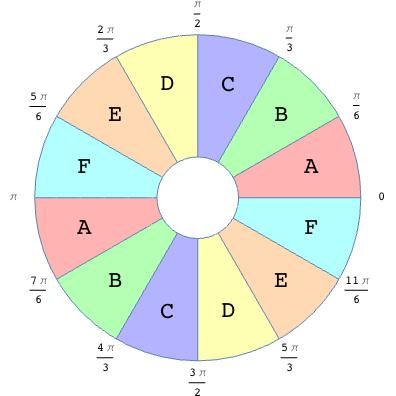
\includegraphics[width = 26mm]{Chapter2/Figs/fRWheel.jpg}} \\
$\fSs[\theta] \otimes \fSe[\theta]$ \\
\end{tabular} &  Factored Rotation : $fR[\thetaA]$ \\ 
\hline \rule[-2ex]{0pt}{5.5ex} 
\bf{A} : $0$& \( \left(\!\!\!

\begin{array}{c}
 1 \\  1 \\ 1\\
\end{array} \!\!\!\right) \otimes \left(\!\!\!
\begin{array}{c}
 1 \\
 \cosine {\thetaA } \\
 \cosine{\Pii{6}-\thetaA } \\
\end{array}

\!\!\!\right) \)& \(  \left(\!\!\!
\begin{array}{ccc}
 1 & 1 & 1 \\
 \fReq{\thetaA } & 1 & \fReq{-\thetaA } \\
 \fReq{\frac{\pi }{6}-\thetaA }& \fReq{\thetaA -\frac{\pi }{6}} & 1 \\
\end{array}
\right) \)  \\ 
\hline \rule[-2ex]{0pt}{5.5ex} \bf{B} : $\frac{\pi}{6}$ & \( \left(\!\!\!

\begin{array}{c}
 1 \\  -1 \\ 1\\
\end{array} \!\!\!\right) \otimes \left(\!\!\!
\begin{array}{c}
 1 \\
 \cosine{\Pii{6}-\thetaA } \\
 \cosine {\thetaA } \\
\end{array}

\!\!\!\right) \)  &  \(  \left(\!\!\!
\begin{array}{ccc}
 1 & 1 & 1 \\
 1 & \fReq{\frac{\pi }{6}-\thetaA } & \fReq{\thetaA -\frac{\pi }{6}} \\
 \fReq{-\thetaA } & \fReq{\thetaA } & 1 \\
\end{array}
\!\!\!\right)  \) \\ 
\hline \rule[-2ex]{0pt}{5.5ex} \bf{C} : $\frac{\pi}{3}$ & \(  \left(\!\!\!

\begin{array}{c}
 1 \\  -1 \\ -1\\
\end{array} \!\!\!\right) \otimes \left(\!\!\!
\begin{array}{c}
 1 \\
 \cosine {\thetaA } \\
 \cosine{\Pii{6}-\thetaA } \\
\end{array}

\!\!\!\right) \)  & \(  \left(\!\!\!
\begin{array}{ccc}
 1 & 1 & 1 \\
 1 & \fReq{-\thetaA } & \fReq{\thetaA } \\
 \fReq{\thetaA -\frac{\pi }{6}} & 1 & \fReq{\frac{\pi }{6}-\thetaA } \\
\end{array}
\!\!\!\right) \)  \\ 
\hline \rule[-2ex]{0pt}{5.5ex} \bf{D}  : $\frac{\pi}{2}$& \( \left(\!\!\!

\begin{array}{c}
 1 \\  1 \\ -1\\
\end{array} \!\!\!\right) \otimes \left(\!\!\!
\begin{array}{c}
 1 \\
 \cosine{\Pii{6}-\thetaA } \\
 \cosine {\thetaA } \\
\end{array}

\!\!\!\right) \)  & \(  \left(\!\!\!
\begin{array}{ccc}
 1 & 1 & 1 \\
 \fReq{\frac{\pi }{6}-\thetaA } & \fReq{\thetaA -\frac{\pi }{6}} & 1 \\
 \fReq{\thetaA } & 1 & \fReq{-\thetaA } \\
\end{array}
\!\!\!\right) \)  \\ 
\hline \rule[-2ex]{0pt}{5.5ex} \bf{E}  : $\frac{2 \pi}{3}$& \(  \left(\!\!\!

\begin{array}{c}
 1 \\  1 \\ 1\\
\end{array} \!\!\!\right) \otimes \left(\!\!\!
\begin{array}{c}
 1 \\
 \cosine {\thetaA } \\
 \cosine{\Pii{6}-\thetaA } \\
\end{array}

\!\!\!\right)\)  & \(  \left(\!\!\!
\begin{array}{ccc}
 1 & 1 & 1 \\
 \fReq{-\thetaA } & \fReq{\thetaA } & 1 \\
 1 & \fReq{\frac{\pi }{6}-\thetaA } & \fReq{\thetaA -\frac{\pi }{6}} \\
\end{array}
\!\!\!\right) \)  \\ 
\hline \rule[-2ex]{0pt}{5.5ex} \bf{F}  : $\frac{5 \pi}{6}$&\( 
\left(\!\!\!

\begin{array}{c}
 1 \\  -1 \\ 1\\
\end{array} \!\!\!\right) \otimes \left(\!\!\!
\begin{array}{c}
 1 \\
 \cosine{\Pii{6}-\thetaA } \\
 \cosine {\thetaA } \\
\end{array}

\!\!\!\right)\)   & \( \left(\!\!\!
\begin{array}{ccc}
 1 & 1 & 1 \\
 \fReq{\thetaA -\frac{\pi }{6}} & 1 & \fReq{\frac{\pi }{6}-\thetaA } \\
 1 & \fReq{-\thetaA } & \fReq{\thetaA } \\
\end{array}
\!\!\!\right)  \)  \\ 
\hline 
\end{tabular} 


We can now relate the functions to each other, since they are now essentially the same function, and $\thetaA$ has the same domain; the values they take have the same range, despite being in different positions in the matrix. This allows us to write the piecewise function $\fR$ independently as a function $\fRO$, which re-orders the elements of the matrix in region $\mathbf{A}$ appropriately for the other regions.

\begin{align}
\fR[\theta] & = \fRO \left[ \fRm{\thetaA} , \theta \right] \\
& = \fRO \left[
\begin{pmatrix}
 1 & 1 & 1 \\
 \text{fRe} (\thetaA)  & 1 & \text{fRe} (-\thetaA ) \\
 \text{fRe} \left(\frac{\pi }{6}-\thetaA \right) & \text{fRe} \left(\thetaA -\frac{\pi }{6}\right) & 1 \\
\end{pmatrix} , \theta \right]
\end{align}

The scaling factor $\fS ( \thetaA )$ can also be further simplified by separating the sign and combining the functional parts.
\begin{align}
\fSe(\theta) 
&=
\begin{cases}
 \left(
\begin{array}{c}
 1 \\
 \cos \left(\frac{\pi }{6}-(\thetaA)\right) \\
 \cos \left((\thetaA)\right) \\
\end{array}
\right) & 
\begin{array}{c}
\frac{\pi }{6}\leq (\theta  \bmod \pi )<\frac{\pi }{3}\lor \\
\frac{\pi }{2}\leq (\theta  \bmod \pi )<\frac{2 \pi }{3}\lor \\
\frac{5 \pi}{6}\leq (\theta  \bmod \pi )<\pi  \\
\end{array} \\
 \left(
\begin{array}{c}
 1 \\
 \cos \left((\thetaA)\right) \\
 \cos \left(\frac{\pi }{6}-(\thetaA)\right) \\
\end{array}
\right)  & 
\begin{array}{c}
0\leq (\theta  \bmod \pi )<\frac{\pi }{6}\lor \\
\frac{\pi }{3}\leq (\theta  \bmod \pi ) < \frac{\pi }{2}\lor \\
\frac{2 \pi }{3}\leq (\theta \bmod \pi ) <\frac{5 \pi }{6} \\
\end{array}
\end{cases} \\
&= 
\left(
\begin{array}{c}
 1 \\
 \cos \left(\frac{\pi }{6}-(\widetilde{\vartheta})\right) \\
 \cos \left(\frac{\pi }{6}-(\widetilde{\theta} )\right) \\
\end{array}
\right) 
\quad \text{where}  \quad 
\begin{array}{c}
\widetilde{\theta} = \theta  \bmod \frac{\pi }{3} \\ 
\widetilde{\vartheta} = \left(\theta - \Pii{6}\right) \bmod \frac{\pi }{3}
\end{array}
\end{align}

then $\fS (\theta) = \fSe (\theta) \otimes \fSs(\theta)$, where $\fSs$ is a piecewise function containing the signs. 

The scaling factors combine in a simple way
\begin{equation}
\nS[\theta] \otimes \rS \otimes \fSe (\theta)   = 
\left(
\begin{array}{c}
 \frac{1}{3}  \\
 \frac{1}{2}\\
 \frac{1}{2} \\
\end{array}
\right)
\end{equation}
The fully factorized matrix can now be written as

\begin{align*}
\nR[\theta] & = \nS[\theta] \otimes \rS \otimes \fSe (\theta) \otimes \fSs(\theta) \otimes\fRO \left[  \fRm{ \thetaA }, \theta \right] \\
& = \left(
\begin{array}{c}
 \frac{1}{3}  \\
 \frac{1}{2}\\
 \frac{1}{2} \\
\end{array}
\right) \otimes \fSs(\theta) \otimes\fRO \left[  \fRm{\thetaA}, \theta \right] \\
\end{align*}

\subsubsection{Quantizing the Rotation}

The factored rotation $\mathbf{fR}$ contains 4 non-integer elements lying between $-1$ and $0$, which we wish to quantize. This can be done simply by multiplying it by $2^{n - 2}$, where $n$ is the bit depth of the integer type, and rounding the result: 

\begin{align}
 \qR[\theta, n] &=
\textbf{Round}\left[
\left(
\begin{array}{c}
 1  \\
 2^{n - 2} \\
 2^{n - 2}  \\
\end{array}
\right)
\bigotimes
\fR[\theta] \right] 
\quad &\text{and} \quad 
\qS[n] &= \left(
\begin{array}{c}
 1  \\
 2^{2-n } \\
 2^{2-n }  \\
\end{array}
\right) 
\end{align}



Since every row in $\fR$ always has an element equal to 1, we will exploit the full range $ -2^{n-2} \le \fR \le 2^{n-2}$ of the integer type. 

\begin{align}
\fR[ \theta ] &= \qS[n]  \otimes \left( \qR[ \theta, n]  + \dqR[ \theta, n ] \right)  \\
                  &= \qS[n]  \otimes \qR[ \theta, n ] +  \dfR[ \theta, n ] 
\end{align}

Thus far, we have assumed that we can achieve a bit depth of two less than the bit depth of the source type for the representation of the rotation matrix. We are now in a position to assess whether the representation introduces any errors.

Given that the source type with a bit depth of $n$, we can work out any errors introduced by finding the difference between using the quantized rotation $\qR$ and the unquantized rotation $\fR$. All the factoring of the rotation is mathematically exact up to and including $\fR$, so any errors that are introduced will be during the rounding.

We are interested in the error introduced by the quantization, so we introduce the perturbation $\dfR[\theta]$ associated with the transform $\fR[\theta]$ produced by the rounding. Defining 

\begin{align*}
\fRe[ \theta ] &=  \qS[ n ]  \otimes  \left( \qRe[ \theta, n ]  + \dqRe[ \theta, n ] \right) 
\end{align*}
because $\qS$ has equal elements in the second and third rows
\begin{equation*}
\fRO \left[ \qS[n] \otimes \mathbf{A} \right] = \qS[n] \otimes \fRO[ \mathbf{A} ]  
\end{equation*}
then
\begin{align*}
\fR[ \theta ] &= \fRO \left[ \fRe[ \theta ] \right] \\
                    &= \fRO \left[ \qS[ n ]  \otimes \left( \qRe[ \theta, n ]  + \dqRe[ \theta, n ] \right) \right]  \\
                   &= \qS[ n ]  \otimes \fRO \left[ \qRe[ \theta, n ]  + \dqRe[ \theta, n ]  \right]  \\
                   &= \qS[ n ]  \otimes \fRO \left[ \qRe[ \theta, n ]   \right]  + \qS[ n ]  \otimes \fRO \left[ \dqRe[ \theta, n ]  \right]  
\end{align*}

The perturbation depends entirely on $\dqRe[\theta,n]$ 

\begin{align*}
\dqRe[\phi] &= \text{Round}\left[ 2^{n-2} \fRe[\phi ] \right]-2^{n-2}\fRe[\phi ] \\
%&= \text{Round}\left[ 2^{n-2} \frac{\um 1}{2} \left(1+\sqrt{3} \tan (\phi )\right)  \right]-2^{n-2}\frac{\um 1}{2} \left(1+\sqrt{3} \tan (\phi )\right) \\
%&= \text{Round}\left[ 2^{n-3} \right]+ \text{Round}\left[ 2^{n-3}\sqrt{3} \tan (\phi ) \right]-2^{n-3}-2^{n-3}\sqrt{3} \tan (\phi )\\
&=  \text{Round}\left[ 2^{n-3}\sqrt{3} \tan (\phi ) \right]-2^{n-3}\sqrt{3} \tan (\phi )\\
\dfRe[\phi] &= 2^{2-n} \dqRe[\phi]  
\end{align*}

The perturbation $\dqR[\theta]$ is a rearrangement of $\dqR[\thetaA] $ 
\begin{align*}
\dqR[\thetaA] &= \fRO[\dqRe, \thetaA ] \\
 &=
\begin{pmatrix}
 0                                     & 0                                   & 0                     \\
 \dqRe[ \thetaA ]              & 0                                   & \dqRe[ -\thetaA ] \\
 \dqRe[ \Pii{6} -\thetaA]   & \dqRe[\thetaA-\Pii{6} ] & 0                     \\
\end{pmatrix}
\end{align*}

The perturbation introduced to each channel is further simplified by recognizing that $\fRe[-\phi]=-1-\fRe[\phi]$, which allows us to find $\dqRe[-\phi]=-\dqRe[\phi]$ i.e. that the sum of the two perturbations in each row equals zero. we can analyze the quantization error in terms of just one function $\dqRe$ and a matrix ordering function $\dqR[\theta] = \fROm \left[ \dqR[ \thetaA ]  \right]$.

\begin{align*}
\dqR[\theta] &= \fROm \left[  
\begin{pmatrix}
 0                                     \\
 \dqRe[ \thetaA ]              \\
 \dqRe[ \Pii{6} -\thetaA]   \\
\end{pmatrix} \otimes
\begin{pmatrix}
 0  &    0  &   0  \\
 1  &    0  & -1  \\
 1  & - 1  &   0  \\
\end{pmatrix}
  ,\theta \right]
\end{align*}


\begin{equation}
\fROm \left[  \left(
\begin{smallmatrix}
 0   & 0   & 0  \\
 a   & 0   & -a \\
 b & - b & 0    \\
 \end{smallmatrix} 
\right)  ,\theta \right] =
\begin{cases}
 \left(
\begin{smallmatrix}
 0 & 0 & 0 \\
 a & 0 & -a \\
 b & -b & 0 \\
\end{smallmatrix} 
\right) & 0\leq (\theta  \bmod \pi )<\frac{\pi }{6} \\
 \left(
\begin{smallmatrix}
 0 & 0 & 0 \\
 0 & b & -b \\
 -a & a & 0 \\
\end{smallmatrix} 
\right) & \frac{\pi }{6}\leq (\theta  \bmod \pi )<\frac{\pi }{3} \\
 \left(
\begin{smallmatrix}
 0 & 0 & 0 \\
 0 & -a & a \\
 -b & 0 & b \\
\end{smallmatrix} 
\right) & \frac{\pi }{3}\leq (\theta  \bmod \pi )<\frac{\pi }{2} \\
 \left(
\begin{smallmatrix}
 0 & 0 & 0 \\
 b & -b & 0 \\
 a & 0 & -a \\
\end{smallmatrix} 
\right) & \frac{\pi }{2}\leq (\theta  \bmod \pi )<\frac{2 \pi }{3} \\
 \left(
\begin{smallmatrix}
 0 & 0 & 0 \\
 -a & a & 0 \\
 0 & b & -b \\
\end{smallmatrix} 
\right) & \frac{2 \pi }{3}\leq (\theta  \bmod \pi )<\frac{5 \pi }{6} \\
 \left(
\begin{smallmatrix}
 0 & 0 & 0 \\
 -b & 0 & b \\
 0 & -a & a \\
\end{smallmatrix} 
\right) & \frac{5 \pi }{6}\leq (\theta  \bmod \pi )<\pi 
\end{cases}
\end{equation}

We can now express the perturbation to the rotation and to the channel elements themselves. The structure of $\fROm$ means that the perturbation to each channel is the product of either $\dqRe[ \thetaA ]$ or $\dqRe[ \Pii{6} -\thetaA]$ with the difference between two of the pixel values. Given that we can assume that the pixel values are positive, being unsigned integers, the extreme values of the perturbation are when one of the two pixel values is zero.  

\begin{align*}
\nR[\theta] & = \nRa[\theta]+\dnR[\theta] \\
& = \nS[\theta] \otimes \rS \otimes \fSe (\theta) \otimes\qS[ n ] \otimes \fSs[\theta]  \otimes \fRO \left[ \qRe[ \theta, n ]  + \dqRe[ \theta, n ]  \right]  \\
& = 
\begin{pmatrix}
 \frac{1}{3}  \\
 \frac{1}{2}\\
 \frac{1}{2} \\
\end{pmatrix}
 \otimes
\begin{pmatrix}
 1  \\
 2^{2-n } \\
 2^{2-n }  \\
\end{pmatrix}
\otimes  \fSs(\theta) \otimes \fRO \left[ \qRe[ \theta, n ]  + \dqRe[ \theta, n ]  \right]   \\
\end{align*}


defining

\begin{align*}
\Scale[\theta, n]   & =
\begin{pmatrix}
  \frac{1}{3} \\
 2^{1-n } \\
 2^{1-n }  \\
\end{pmatrix}
\otimes  \fSs(\theta)    \\
\nRa[\theta]   & =  \Scale[\theta] \otimes \fRO \left[   \qRe[ \theta, n ] \right]   \\
\dnR[\theta]   & =  \Scale[\theta] \otimes \fRO \left[ \dqRe[ \theta, n ] \right] \\
\end{align*}

\newcommand{\rgb}{\vec{v}}
\newcommand{\w}{\vec{w}}
\newcommand{\dW}{\vec{\delta w}}

the perturbation to the rotated channel elements $\dW$ is found for an input set of pixel values $\rgb= 2^n\normed{\rgb} $


\begin{align*}
\w+\dW &= \nRa[\theta] \cdot \rgb+\dnR[\theta] \cdot \rgb \\
\dW &= 2^n\dnR[\theta] \cdot \normed{\rgb} \\
        &= 2^n\Scale[\theta] \otimes \fRO \left[ \dqRe[ \theta, n ] \right] \cdot \normed{\rgb} \\
        &= \fROm \left[  
        \begin{pmatrix}
         0                                     \\
         2 \dqRe[ \thetaA ]              \\
         2 \dqRe[ \Pii{6} -\thetaA]   \\
        \end{pmatrix} \otimes
        \begin{pmatrix}
         0  &    0  &   0  \\
         1  &    0  & -1  \\
         1  & - 1  &   0  \\
        \end{pmatrix}
          ,\theta \right]
\end{align*}

So, to minimize the perturbation, we need to simultaneously minimize $\pm 2 \dqRe[ \thetaA ]  $ and $\pm 2 \dqRe[ \Pii{6} -\thetaA]$


%\begin{figure}[h!]
%  \centering
%    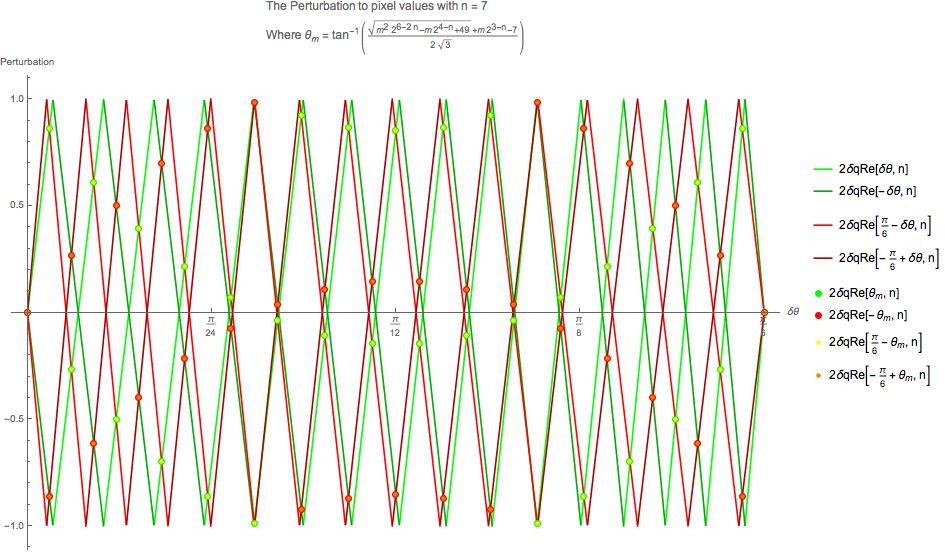
\includegraphics[width=0.99\textwidth]{Chapter2/Figs/PtbToChanBoth.jpg}
%    \caption{Perturbation in the chromatic channels.}  \label{fig:PtbToChan}
%\end{figure}


\begin{sidewaysfigure}[p]
  \centering
    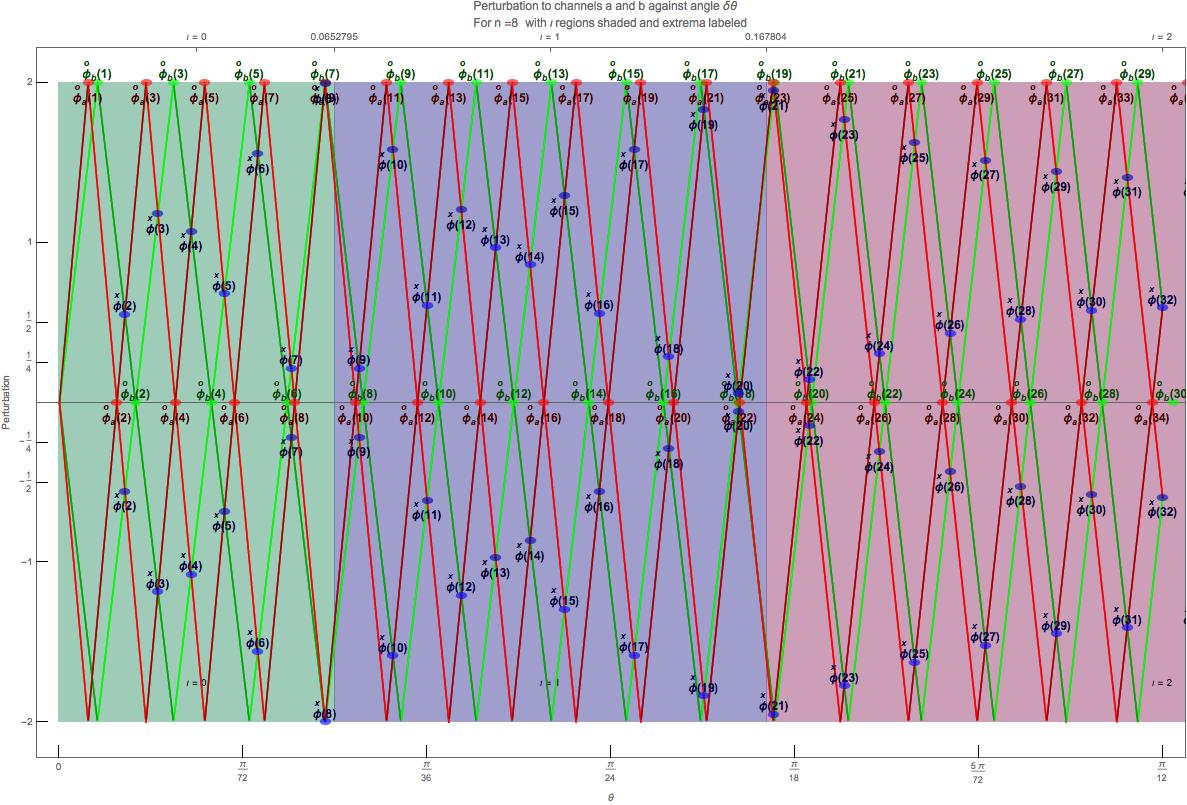
\includegraphics[width=0.99\textwidth]{Chapter2/Figs/PtbToChanBothWithPoints.jpg}
    \caption{ Perturbation to channels a and b against angle $\delta \theta$ \\
    For n = 8  with $\iota$ regions shaded and extrema labelled }  \label{fig:PtbToChan}
\end{sidewaysfigure}

The maxima for each function are where $\pm 2 \dqRe[ \thetaA ]  = \pm 1$ and $\pm 2 \dqRe[ \Pii{6} -\thetaA]= \pm 1$, and the minima are where $\pm 2 \dqRe[ \thetaA ]  = 0$ and $\pm 2 \dqRe[ \Pii{6} -\thetaA] = 0$. To find the corresponding values of $\thetaA$, all that is needed is an inverse function for $\dqRe$. In essence $\dqRe[\phi]$ discretizes $\sqrt{3} \tan (\phi )$ into steps of $2^{3-n}$. The minima can be found by taking the inverse of $\sqrt{3} \tan (\phi )$, given that
$0\le\sqrt{3} \tan (\phi )\le1$ for $0 \le \phi \le \Pii{6}$ we can say that $\text{Round}\left[ 2^{n-3}\sqrt{3} \tan (\phi ) \right] \in \{ 0, 1, 2, \cdots 2^{n-3} \}$ 


\begin{align*}
\dqRe[\phi] & = 0 & \dqRe[\Pii{6}-\phi] & = 0 \quad \text{when} \\
% 2^{n-3}\sqrt{3} \tan (\phi ) &= \text{Round}\left[ 2^{n-3}\sqrt{3} \tan (\phi ) \right]  & 
% 2^{n-3}\sqrt{3} \tan (\Pii{6}-\phi ) &= \text{Round}\left[ 2^{n-3}\sqrt{3} \tan (\Pii{6}-\phi ) \right]\\
2^{n-3}\sqrt{3} \tan (\phi ) & = m & 
2^{n-3}\sqrt{3} \tan (\Pii{6}-\phi ) &= m \quad \text{where}\quad m=0,1,2 \cdots 2^{n-3} \\
 \check{\phi}_{b} = & \arctan\left(\frac{m 2^{3-n}}{\sqrt{3}}  \right) &
 \check{\phi}_{a} = & \arctan\left(\frac{2 \sqrt{3} m}{2^n - 2 m}\right) 
\end{align*}

The maxima can be found by recognizing that the maximum rounding error is a half and evaluating at these points

\begin{align*}
\dqRe[\hat{\phi}_{b} ] & = \pm 1 & \dqRe[\Pii{6}-\hat{\phi}_{a} ] & = \pm 1  \quad \text{when} \\
\hat{\phi}_{b} & =\arctan\left(\frac{ 2^{3-n} }{\sqrt{3}} \left(m+\frac{1}{2}\right) \right) &
\hat{\phi}_{a} & = \arctan\left(\frac{2 \sqrt{3} \left(m+\frac{1}{2}\right)}{2^n - 2 \left(m+\frac{1}{2}\right)}\right)  \\
 \hat{\phi}_{b}  &=  \arctan\left(\frac{(2 m+1) 2^{2-n}}{\sqrt{3}}          \right) &
  \hat{\phi}_{a}  &=  \arctan\left(\frac{\sqrt{3} (2 m+1)}{2^n-2 m-1}  \right) \\
  \quad&\text{with}\quad   m =  0,1,2,3 \cdots2^{n-3}-1 
\end{align*}

We are interested in a compromise between the perturbations to each channel which is where the perturbations intersect. It would be useful to be able to assign a relative importance $\alpha$ and $\beta$ to each channel a and b respectively. 
\begin{gather*}
\beta \; \dqRe[\phi] = \alpha \; \dqRe[\frac{\pi}{6} -\phi]  \quad \textbf{when} \\
\begin{split}
\beta \text{Round}\left[ 2^{n-3}\sqrt{3} \tan (\phi ) \right] - \alpha \text{Round}\left[ 2^{n-3}\sqrt{3} \tan (\frac{\pi}{6} - \phi ) \right] \\
=   2^{n-3} \left(\sqrt{3} \alpha  \tan (\theta ) + 2 \beta  \sin (\theta ) \sec \left(\frac{\pi }{6}-\theta \right)\right)
\end{split}
\end{gather*}

The values $\alpha$ and $\beta$ can only move the point of intersection within the bounds of the extrema. Therefore, any solution for the point of intersection will enable the bounding extrema to be identified. 

We solve first for the case where $\alpha=1$ and $\beta=1$. Recognizing that the rounded part can only take certain values
\begin{gather*}
i =  \text{Round}\left[ 2^{n-3}\sqrt{3} \tan (\phi ) \right] - \text{Round}\left[ 2^{n-3}\sqrt{3} \tan (\frac{\pi}{6} - \phi ) \right]
 \quad \text{where}\quad i=0,1,2 \cdots 2^{n-2}
 \end{gather*}
then

\newcommand{\thetaX}[1]{\overset{\times}{\phi}\left( \scalebox{0.75}[1.0]{\( #1 \)}\right)}

\begin{gather*}
\thetaX{i}=\arctan\left(\frac{\sqrt{i^2 2^{6-2 n}-i 2^{4-n}+49}+i 2^{3-n}-7}{2 \sqrt{3}}\right) \quad \text{where}\quad i=0,1,2 \cdots 2^{n-2}
\end{gather*}

Each point of intersection is defined and bounded by 4 extrema. Comparing with the functional form of the extrema allows these 4 points to be identified.
%
%\begin{align*}
% \check{\phi}_{a} = & \arctan\left(\frac{2m \sqrt{3} }{2^n - 2 m}\right) &
% \check{\phi}_{b} = & \arctan\left(\frac{2m 2^{2-n}}{\sqrt{3}}       \right) \\ 
% & \text{with}\quad   m =  0,1,2,3 \cdots2^{n-3} \\
% \hat{\phi    }_{a}  = & \arctan\left(\frac{\sqrt{3} (2 m+1)}{2^n-(2 m+1)}  \right) &
% \hat{\phi   }_{b}  = & \arctan\left(\frac{(2 m+1) 2^{2-n}}{\sqrt{3}}          \right) \\
% &\text{with}\quad   m =  0,1,2,3 \cdots2^{n-3}-1 
%\end{align*}
%

\newcommand{\extremaTheta}[2]{\mathring{\phi} _{#1}\left( \scalebox{0.75}[1.0]{\( #2 \)}\right)}

\begin{align*}
 \extremaTheta{a} {l}= & \arctan\left(\frac{l \sqrt{3} }{2^n - l}\right) &
 \extremaTheta{b} {l}= & \arctan\left(\frac{l \; 2^{2-n}}{\sqrt{3}}       \right) \\ 
 \check{\phi}_{a} = & \extremaTheta{a} {2m} &
 \check{\phi}_{b} = & \extremaTheta{b} {2m} 
 & \text{with}\quad   m =  0,1,2,3 \cdots2^{n-3} \\
  \hat{\phi}_{a} = & \extremaTheta{a} {2m+1} &
  \hat{\phi}_{b} = & \extremaTheta{b} {2m+1} 
 &\text{with}\quad   m =  0,1,2,3 \cdots2^{n-3}-1 
\end{align*}

%\begin{tabular}{|c|c|c|c|}
%\hline
%  & Channel a & Channel b &  m \\ 
%\hline Minima  &  $ \check{\phi}_{a}(m)  =  \extremaTheta{a}{2m}  $ & $ \check{\phi}_{b}(m)  = \extremaTheta{b}{2m}  $ &  $m \in \{ 0,1,2,3 \cdots2^{n-3}  \} $\\ 
%\hline Maxima  &  $ \hat{\phi}_{a}(m)  = \extremaTheta{a}{2m+1}   $ & $ \hat{\phi}_{b}(m)  = \extremaTheta{b}{2m+1}  $  & $ m \in \{ 0,1,2,3 \cdots2^{n-3} -1 \}  $ \\ 
%\hline 
%\end{tabular} 

Separating the points of intersection into even and odd terms facilitates the identification. 

\begin{tabular}{|c|c|c|c|}
\hline
  & Channel a & Channel b &  i \\ 
\hline Minima  &  $ \check{\phi}_{a}(\frac{i}{2})=\extremaTheta{a}{i} $ & $ \check{\phi}_{b}(\frac{i}{2})=\extremaTheta{b}{i} $ & $ i \in \{0,2,4,6\cdots2^{n-2} \} $\\ 
\hline Maxima  &  $     \hat{\phi}_{a}(\frac{i-1}{2})=\extremaTheta{a}{i} $ & $     \hat{\phi}_{b}(\frac{i-1}{2})=\extremaTheta{b}{i} $ & $ i \in \{1,3,5,7\cdots2^{n-2}-1\}  $ \\ 
\hline 
\end{tabular} 


The following ranges are guaranteed to be true for even or odd values of $i$, with very specific values of $p$ and $q$.
%
%\begin{align*}
%\begin{array}{cc}
%  \extremaTheta{b}{p} & < \\
%  \extremaTheta{a} {q-1} & < 
%\end{array}
%&\thetaX{i} 
%\begin{array}{cc}
%  < & \extremaTheta{a}{q}  \\
%  < & \extremaTheta{b}{p+1}  
%\end{array} 
%& \bigvee
%\begin{array}{cc}
%  \extremaTheta{a}{q} & < \\
%  \extremaTheta{b} {p+1} & < 
%\end{array}
%&\thetaX{i+1}
%\begin{array}{cc}
%  < & \extremaTheta{b}{p+2}  \\
%  < & \extremaTheta{a}{q+1}  
%\end{array} & 
%\begin{array}{cc}
%p &\in \{ 2 \mathbb{N} +1 \}  \\
%q &\in \{ 2 \mathbb{N} +1 \}  \\
%i  &\in \{ 2 \mathbb{N} +1 \}
%\end{array}
%\end{align*}


\begin{align*}
\begin{array}{cc}
  \extremaTheta{b}{p-1} & < \\
  \extremaTheta{a} {q} & < 
\end{array}
&\thetaX{i} 
\begin{array}{cc}
  < & \extremaTheta{a}{q+1}  \\
  < & \extremaTheta{b}{p}  
\end{array} 
& \bigvee
\begin{array}{cc}
  \extremaTheta{a}{q+1} & < \\
  \extremaTheta{b} {p} & < 
\end{array}
&\thetaX{i+1} 
\begin{array}{cc}
  < & \extremaTheta{b}{p+1}  \\
  < & \extremaTheta{a}{q+2}  
\end{array} & 
\begin{array}{cc}
p  &\in \{ 2 \mathbb{N}  \}  \\
q  &\in \{ 2 \mathbb{N}  \}  \\
2  & \le i  \le 2^{n-2} -1
\end{array}
\end{align*}

\newcommand{\meanIndx}{\overline{\mathbf{i}}}

This slightly glib definition illustrates the pattern for the extrema bounding the points of intersection. At the start of a $\frac{\Pi}{6}$ region, i.e. for low values of $i$, $p=i$ and $q=i$. The maxima swap orderings between certain values of $i$ within a $\frac{\Pi}{6}$ region. This is evident in the inescapable indices of $i-1$ and $i+1$, regardless of the starting values for $i$ for either the maxima or minima. So, whilst it is true that $\extremaTheta{a} {i} > \extremaTheta{b} {i}$, it is not always true that $\extremaTheta{a} {i+1} > \extremaTheta{b} {i-1}$. This leads to the question of what happens when this boundary $\extremaTheta{a} {i+1} = \extremaTheta{b} {i-1}$ is crossed. Firstly, the even-odd ordering (i.e. the a-b channel ordering) is flipped; secondly, the indices are shifted. A second transition restores the a-b ordering and shifts the indices again. As the index $i$ passes the half way point $\meanIndx = 2^{n-3}$, the transitions occur in the opposite direction, restoring the indices and ordering. Transitions occur where $i$ satisfies $\extremaTheta{a} {i+\iota} = \extremaTheta{b} {i-\iota}$, with $\iota \in \{ 1,2,3 \cdots \left(7-4 \sqrt{3}\right) 2^{n-3}\} $. 

\begin{gather*}
\meanIndx = 2^{n-3} \qquad
\varGamma(\iota, n) = \sqrt{\iota ^2 - 14 \iota \meanIndx + \meanIndx^{2} } 
\end{gather*}

The region $\iota$ for a given value of $i$ is the highest value of $\iota$ for which the following condition remains true:

\begin{gather*}
\meanIndx -\varGamma(\iota, n) \leq i \leq \varGamma(\iota, n) + \meanIndx 
\end{gather*}

For a given value of $\theta$ and $n$, we can find the intersection index $i$, and from this we can find $\iota$:

\begin{gather*}
i(\delta\theta, n) = \frac{\meanIndx \tan (\delta \theta ) \left(\sqrt{3} \tan (\delta \theta )+7\right)}{\tan (\delta \theta )+\sqrt{3}} 
\quad \text{where} \quad \delta\theta = \theta \mod{\frac{\pi}{6} }\\
 \iota(i,n)  = \left\lfloor 7\ \meanIndx-\sqrt{i^2 - 2 i \; \meanIndx + 49\ \meanIndx^2 }\right\rfloor 
\end{gather*}

The sequence of a-b channel extrema depends on both the index $i$ and the region $\iota$ in the following way:

\begin{align*}
\begin{array}{cc}
  \extremaTheta{b}{i-\iota-1} & < \\
  \extremaTheta{a} {i+\iota} & < 
\end{array}
&\thetaX{i}
\begin{array}{cc}
  < &  \extremaTheta{a}{i+\iota+1}  \\
  < & \extremaTheta{b}{i-\iota}  
\end{array} & \text{when} \quad 
\begin{array}{lcl}
i \in \{2 \mathbb{N}+1\}  & \land & \iota \in \{2 \mathbb{N}+1\} \  \lor \\ 
i \in \{2 \mathbb{N}     \} &  \land & \iota \in \{2 \mathbb{N}    \} \\
 \end{array}  \\
\begin{array}{cc}
  \extremaTheta{a}{i+\iota} & < \\
  \extremaTheta{b} {i-\iota-1} & < 
\end{array}
&\thetaX{i}
\begin{array}{cc}
  < & \extremaTheta{b}{i-\iota}  \\
  < & \extremaTheta{a}{i+\iota+1}  
\end{array} & 
\text{when} \quad 
\begin{array}{lcl}
 (i\in \{2 \mathbb{N}+1\} & \land & \iota \in \{2 \mathbb{N}    \}) \ \lor \\
 (i\in \{2 \mathbb{N}    \} & \land & \iota \in \{2 \mathbb{N}+1\})
 \end{array} 
\end{align*}

%The other two ranges can swap direction around the central value  $\overline{m}$ in a region governed by $\Gamma$ which is the distance from $\overline{m}$ at which the order of the extrema switch between channels.
%
%\begin{gather*}
%\overline{m}=\frac{1}{2} \left(2^{n-3}-1\right) \qquad
%\varGamma(n)=\frac{1}{2} \sqrt{2^{2 (n-3)}-14\ 2^{n-3}+1} \\
%\hat{L}(m)=\begin{cases}
%< & \quad    m <   \bar{m} -\Gamma \vee m > \bar{m} + \Gamma   \\
%> & \quad  \bar{m} - \Gamma \leq m \leq \bar{m} + \Gamma \\
%\end{cases} \\
%\end{gather*}
%defining a relational operator which depends on $\hat{L}(m)$ 
%\begin{align}
%\gtrless &= \hat{L}(\scriptsize{m-\frac{1}{2}}) & \lessgtr &= \hat{L}(\scriptsize{m})  
%\end{align}
%allows the bounds for the points of intersection to be concisely written
%%\begin{alignat*}{5}
%% \hat{\phi}_{b}(m-1) && \gtrless  && \thetaX{}(2m)       &&\gtrless  &&     \hat{\phi}_{a}(m)  \\
%% \check{\phi}_{b}(m)  && \lessgtr                   && \thetaX{}(2m+1)  && \lessgtr                  &&\check{\phi}_{a} (m+1) 
%%\end{alignat*}
%
%
%
%
%\begin{align}
%\begin{array}{cc}
% \hat{\phi}_{b}(m-1) &\gtrless \\
%  \check{\phi}_{a} (m) & < 
%\end{array}
%\thetaX{2m}
%\begin{array}{cc}
%\gtrless &     \hat{\phi}_{a}(m)  \\
%  < & \check{\phi}_{b}(m)  
%\end{array} \quad
%& \quad
%\begin{array}{cc}
%      \hat{\phi}_{a}(m)  & <            \\
% \check{\phi}_{b}(m)  & \lessgtr   
%\end{array}
%\thetaX{2m+1}
%\begin{array}{cc}
% <             &    \hat{\phi}_{b}(m)  \\
%\lessgtr    &\check{\phi}_{a} (m+1)  
%\end{array} 
%\end{align}
%
%Adjusting for the intersection index $i$ allows us to see that the intersection points are best classified by being either odd or even values of $i$
%%
%%\begin{align}
%%\begin{array}{cc}
%% \hat{\phi}_{b}(\frac{i}{2}-1) &\gtrless \\
%%  \check{\phi}_{a} (\frac{i}{2}) & < 
%%\end{array}
%%\thetaX{i} 
%%\begin{array}{cc}
%%\gtrless &     \hat{\phi}_{a}(\frac{i}{2})  \\
%%  < & \check{\phi}_{b}(\frac{i}{2})  
%%\end{array} \quad
%%& \quad
%%\begin{array}{cc}
%%      \hat{\phi}_{a}(\frac{i}{2})  & <            \\
%% \check{\phi}_{b}(\frac{i}{2})  & \lessgtr   
%%\end{array}
%%\thetaX{i+1}
%%\begin{array}{cc}
%% <             &    \hat{\phi}_{b}(\frac{i}{2})  \\
%%\lessgtr    &\check{\phi}_{a} (\frac{i}{2}+1)  
%%\end{array} 
%%\end{align}
%%
%%\begin{align}
%%\begin{array}{cc}
%% \hat{\phi}_{b}(\frac{i}{2}-1) &\gtrless \\
%%  \check{\phi}_{a} (\frac{i}{2}) & < 
%%\end{array}
%%\thetaX{i} 
%%\begin{array}{cc}
%%\gtrless &     \hat{\phi}_{a}(\frac{i}{2})  \\
%%  < & \check{\phi}_{b}(\frac{i}{2})  
%%\end{array} \quad
%%& \quad
%%\begin{array}{cc}
%%      \hat{\phi}_{a}(\frac{i-1}{2})  & <            \\
%% \check{\phi}_{b}(\frac{i-1}{2})  & \lessgtr   
%%\end{array}
%%\thetaX{i} 
%%\begin{array}{cc}
%% <             &    \hat{\phi}_{b}(\frac{i-1}{2})  \\
%%\lessgtr    &\check{\phi}_{a} (\frac{i-1}{2}+1)  
%%\end{array} 
%%\end{align}
%%
%%\begin{align*}
%%\thetaX{i}  \in & \begin{cases}
%%\begin{array}{cc}
%% \hat{\phi}_{b}(\frac{i}{2}-1) &\gtrless \\
%%  \check{\phi}_{a} (\frac{i}{2}) & < 
%%\end{array}
%%\thetaX{i} 
%%\begin{array}{cc}
%%\gtrless &     \hat{\phi}_{a}(\frac{i}{2})  \\
%%  < & \check{\phi}_{b}(\frac{i}{2})  
%%\end{array} & 
%%i \in \{ 2 \mathbb{N} \} \\
%%\begin{array}{cc}
%%      \hat{\phi}_{a}(\frac{i-1}{2})  & <            \\
%% \check{\phi}_{b}(\frac{i-1}{2})  & \lessgtr   
%%\end{array}
%%\thetaX{i} 
%%\begin{array}{cc}
%% <             &    \hat{\phi}_{b}(\frac{i-1}{2})  \\
%%\lessgtr    &\check{\phi}_{a} (\frac{i-1}{2}+1)  
%%\end{array}  & 
%%i \in \{ 2 \mathbb{N} +1 \}
%%\end{cases}
%%\end{align*}
%
%
%\begin{align*}
%\begin{array}{cc}
% \extremaTheta{b}(i-1) &\gtrless \\
% \extremaTheta{a}(i)     & < 
%\end{array}
%& \thetaX{i}
%\begin{array}{cc}
%\gtrless & \extremaTheta{a}(i+1)  \\
% <          & \extremaTheta{b}(i)  
%\end{array} & 
%i &\in \{ 2 \mathbb{N} \}  & \gtrless &= \hat{L}\left( \frac{i-1}{2} \right)   \\
%\begin{array}{cc}
% \extremaTheta{a}(i)  & <            \\
% \extremaTheta{b}(i-1)  & \gtrless  
%\end{array}
%& \thetaX{i} 
%\begin{array}{cc}
% <             &  \extremaTheta{b}(i)  \\
%\gtrless    &  \extremaTheta{a} (i+1)  
%\end{array}  & 
%i &\in \{ 2 \mathbb{N} +1 \} 
%\end{align*}

We want to classify the points of intersection as greater or lesser than a tolerance $0 < \tau \le 1$. In order to do this, we make a linear approximation to the perturbation between the extrema. There is one point of intersection between each of the maxima and corresponding minima. A bit of geometry allows us to write a classification criteria for each of the points of intersection.

Defining a function for the degree of error at the point of intersection using the linear approximation from the four extrema surrounding the point, and generalizing to allow for different maximum errors $\alpha$ for channel $a$ and $\beta$ for channel b
\begin{align*}
h(i,\iota) & =
\frac{\alpha  \beta  (\extremaTheta{a} {i+\iota }-\extremaTheta{b} {i-\iota })}
{\beta  (\extremaTheta{a} {i+\iota } - \extremaTheta{a} {i+\iota +1} ) + \alpha  (\extremaTheta{b} {i-\iota -1} - \extremaTheta{b} {i-\iota } ) }  & \text{when} \quad 
\begin{array}{lcl}
i \in \{2 \mathbb{N}+1\}  & \land & \iota \in \{2 \mathbb{N}+1\} \  \lor \\ 
i \in \{2 \mathbb{N}     \} &  \land & \iota \in \{2 \mathbb{N}    \} \\
 \end{array}  \\
h(i,\iota) & =
\frac{\alpha  \beta  (\extremaTheta{b} {i-\iota -1}-\extremaTheta{a} {i+\iota +1})}
{\beta  ( \extremaTheta{a} { i+\iota } -\extremaTheta{a} { i+\iota + 1 } ) +\alpha  ( \extremaTheta{b} {i-\iota -1} -\extremaTheta{b} {i-\iota } ) }  & \text{when} \quad 
\begin{array}{lcl}
i \in \{2 \mathbb{N}   \}  & \land & \iota \in \{2 \mathbb{N} + 1\} \  \lor \\ 
i \in \{2 \mathbb{N}  +1 \} &  \land & \iota \in \{2 \mathbb{N}    \} \\
 \end{array}  
\end{align*}

allows the criteria for a channel to be written as $\tau \ge h(i,\iota)$. 

\parpic(79mm,104mm)[r]{\fbox{\parbox{76mm}{
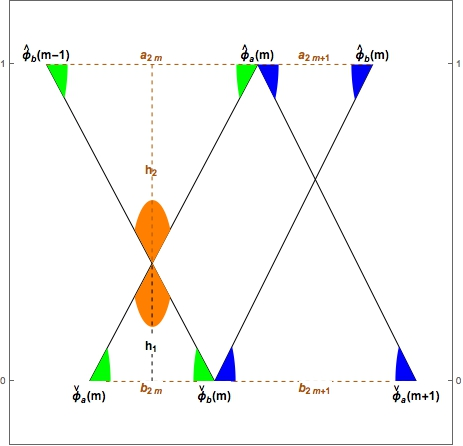
\includegraphics[width=76mm]{Chapter2/Figs/GeometryClassifyPoint.jpg}  \\
\centering  $\frac{h_1}{h_2} = \frac{b}{a} \quad h_1 = \frac{b}{a+b} $ \\
\centering $a_{2m}  =     \| \hat{\phi}_{b}(m-1) -     \hat{\phi}_{a}(m) \|  $ \\
\centering $b_{2m}  = \check{\phi}_{a}(m)     - \check{\phi}_{b}(m)$ \\
\centering $a_{2m+1}   =     \hat{\phi}_{a}(m)     -      \hat{\phi}_{b}(m)$    \\   
\centering $b_{2m+1}  = \| \check{\phi}_{b}(m)     - \check{\phi}_{a} (m+1) \| $  \\
}}
}

The criteria $\tau =\text{\textonehalf}$ with $\alpha=\beta$ selects from either the odd values or the even values of i, because if $h(i,n)<\text{\textonehalf}$ is true, then $h(i+1,n)<\text{\textonehalf}$  is false and vice versa. There are $2^{n-2}$ points of intersection and $2^{n-3}$ which satisfy the criteria $\tau = \frac{1}{2}$. The algorithm as implemented in openCV leaves the decision about the criteria up to the programmer. The programmer chooses a value for $\theta$ and selects a value for $\tau$. The algorithm returns the nearest value of $\theta$ which satisfies the condition defined by $\tau$. The programmer then decides whether the suggested value for $\theta$ is acceptable and either adopts the suggested value, or chooses a value as close as possible, accepting the possibility of errors.

For example, in this project $n$ is 8, so $\intR \in \{ -2^{8-2} \cdots 2^{8-2} \}$, which gives $2^{8-3}-1$ values in each $\frac{\pi}{6}$ region, producing a maximum perturbation of less than \textonehalf. In total, there are $12 (2^{8-3}-1) = 372$ possible values for $\theta$ which produces a maximum perturbation of less than \textonehalf. This would allow the destination pixel values to be expressed in 8-bit numbers without error using a transformation matrix expressed in 6-bit signed integers. The statistics performed to determine $\theta$ are not demanding enough to justify rejecting a suggested value of theta within 1\textdegree  of the requested value. It is, however, important to know the value actually used in the algorithm, which is why the mechanism for adjusting $\theta$ is separate from the color-space algorithm and is under the control of the programmer. For instance, in the implementation below, the suggested value is accepted and used to adjust the statistical model, keeping all the values in correct correspondence.

%\hrule
%
%this is junk which needs to be put in line with the succeeding section.
%
%\begin{equation}
%\intR =
%\text{int}\left(
%\left(
%\begin{array}{c}
% 1 \\
% 2^{1-n_2} \; \tRange_2\\
% 2^{1-n_3} \; \tRange_3 \\
%\end{array}
%\right) 
%\bigotimes
%\left(
%\begin{array}{ccc}
% 1 & 1 & 1 \\
% -\sin \left(\theta +\Pii{6}\right) &  \cos (\theta ) &  \sin \left(\theta -\Pii{6}\right) \\
% -\cos \left(\theta +\Pii{6}\right) & - \sin (\theta ) & \cos \left(\theta -\Pii{6}\right) \\
%\end{array}
%\right)
%\right)
%\end{equation}
%
%\begin{equation}
%\widehat{R}_{xyz}(\theta,\mu,\sigma) =
%\left(
%\begin{array}{c}
% \frac{\min\left\{\Delta(\mu_1,\sigma_1), 1 \right\}}{\sqrt{3}}  \\
% \sqrt{\frac{2}{3}} \frac{\min\left\{\Delta(\mu_2,\sigma_2), 1 \right\} }{2^{1-n_2} \; \tRange_2} \\
% \sqrt{\frac{2}{3}} \frac{\min\left\{\Delta(\mu_3,\sigma_3), 1 \right\}}{2^{1-n_3} \; \tRange_3} \\
%\end{array}
%\right) 
%\bigotimes
%\intR 
%\end{equation}
%
%using $\tRange(\theta,\mu,\sigma) = \min\left\{\Delta(\mu,\sigma), 1 \right\} \srcRange \mathbf{L}(\theta) $
%\begin{equation}
%\widehat{R}_{xyz}(\theta,\mu,\sigma) =
%\left(
%\begin{array}{c}
% \frac{\min\left\{\Delta(\mu_1,\sigma_1), 1 \right\}}{\sqrt{3}}  \\
% \sqrt{\frac{2}{3}} \frac{1}{2^{1-n_2} \; \srcRange \text{L}_2(\theta)} \\
% \sqrt{\frac{2}{3}} \frac{1}{2^{1-n_3} \; \srcRange \text{L}_3(\theta)} \\
%\end{array}
%\right) 
%\bigotimes
%\intR 
%\end{equation}
%
%\begin{equation}
%\widehat{R}_{xyz}(\theta,\mu,\sigma) =
%\left(
%\begin{array}{c}
%\min\left\{\Delta(\mu_1,\sigma_1), 1 \right\} \\
%\min\left\{\Delta(\mu_2,\sigma_2), 1 \right\}  \\
%\min\left\{\Delta(\mu_3,\sigma_3), 1 \right\}  \\
%\end{array}
%\right)
%\bigotimes
%\left(
%\begin{array}{c}
% \frac{1}{\sqrt{3}} \\
% \sqrt{\frac{2}{3}}  \\
% \sqrt{\frac{2}{3}} \\
%\end{array}
%\right) \bigotimes
%\left(
%\begin{array}{c}
% 1 \\
% \frac{1}{2^{1-n_2} \; \tRange_2} \\
% \frac{1}{2^{1-n_3} \; \tRange_3} \\
%\end{array}
%\right) 
%\bigotimes
%\text{int}\left(
%\left(
%\begin{array}{c}
% 1 \\
% 2^{1-n_2} \; \tRange_2\\
% 2^{1-n_3} \; \tRange_3 \\
%\end{array}
%\right) 
%\bigotimes
%\left(
%\begin{array}{ccc}
% 1 & 1 & 1 \\
% -\sin \left(\theta +\Pii{6}\right) &  \cos (\theta ) &  \sin \left(\theta -\Pii{6}\right) \\
% -\cos \left(\theta +\Pii{6}\right) & - \sin (\theta ) & \cos \left(\theta -\Pii{6}\right) \\
%\end{array}
%\right)
%\right)
%\end{equation}
%
%All that remains is to determine if the statistics allow for a reduced representation of the rotation. An equtaion for the boundary of the one to one fidelity region must be found in the source color space and then checked against the conditions given above \ref{eq:errorFreeConditions}. 

\section{Preservation of Color Information}\label{sec:PreservationOfColorInformation}

The goal of the algorithm is to preserve all the information captured by the camera which relates to skin whilst discarding as much of the irrelevant information as possible. Given that edges and features often present as shadows and highlights, all the information captured in terms of luminosity will be regarded as relevant information, at least as far as the manipulation of individual pixel values is concerned. Considering the chromatic information, the importance of the pixel value will be directly determined by a Gaussian distribution.

Knowing the range of values produced by the rotation allows us to scale the transformation to fit into the range of the destination data type. If we have RGB pixel values in a given machine data type, the amount of information contained in each of those channels is equal to the number of values accessible in that data type. For example: for 8-bit, unsigned integers, there are 256 possible values. After a rotation, we are interested in the amount of information which lies along the new axes. This is found simply by multiplying the range of the source data type by the length of the new axes found for the unit cube. To preserve all the information captured, we would therefore have to use a larger data type to store the new values. We are, however, only interested in a small region in the chromatic space. The question is, then, how to preserve the relevant information in a way consistent with the significance indicated by the aforementioned Gaussian distribution.


None of the rotated axes have lengths less than 1 for the unit RGB cube. For this reason we've written redistribution functions which perform any necessary type conversion whilst preserving the information in a controlled way; we can keep the information where it's needed and discard it where it's irrelevant. So although this is strictly beyond the normal meaning of a color space conversion, it is addressing a connected issue and belongs in the conversion. In terms of optimization, it is also the most efficient place in the code in which to perform this adjustment, allowing us to --- for the sake of example --- discard the details of the colors of a duck's feathers whilst keeping the hues and tones of human skin.

We can use a function to redistribute the information contained on the longer axis onto the shorter axis, which can be expressed in the discrete representation of that axis necessitated by internal integer data types. There are three ways in which to implement the redistribution functions:

\subsection{Partition}\label{sec:Partition}

The most straightforward redistribution method is to simply preserve the information in a 1-to-1 fashion within a region. The region can be defined in terms of the distribution Gaussian by specifying a significance level in terms of the variance or the standard deviation.

\subsection{Linear}\label{sec:Linear}

A slightly more sophisticated method is to use a linear redistribution. A linear distribution is equivalent to partitioning given a unit gradient. However, a linear redistribution function allows for the possibility of data compression. So then, in the case where the region of interest contains more information than can be expressed in the destination data type, a linear distribution function allows an even compression of the information from source to destination. ~\cite{Lee2002}

\subsection{ERF (Gaussian Error Function)}\label{sec:ERF}

The integral of the cumulative Gaussian (i.e. Error Function) allows the redistribution of the information on the axis in a way which selectively preserves the information about a point on the axis (i.e. the mean of the Gaussian), and then progressively discard the information as it falls into the tails of the Gaussian. So, it provides a non-linear distribution of the information. The Gaussian can be seen as describing our interest in the information contained along the axis, so it's logical to use the error function to redistribute the information. The disadvantage of this is simply the computational effort involved in generating the error function.

The error function distribution is mathematically correct, being directly related to the Gaussian fit. Computationally, there are two considerations: the numerical representation, and performance. The discrete representation of the numerics means that --- for a significant number of possible distributions --- distributing using the error function has little to no advantage (or indeed difference) from using a linear distribution.

Considering the preservation of information captured, mappings with a gradient greater than 1 are undesirable because they preserve all the information whilst being informatically wasteful in that there are functionally inaccessible discrete values in the destination range. Our stated aim is to preserve the information in the image pertaining to human skin; unevenly distributing this information across a discrete data type is not only wasteful in terms of memory, but also of processing resources because subsequent processing routines will treat the data as if it has a higher fidelity than it actually does.

To construct a distribution function, we first need to describe the relationship of the error function to the Gaussian fit, and then produce a function with the appropriate range and domain. For a Gaussian fit with an amplitude A, a mean of $\mu$, and a standard deviation of $\sigma$, where $\mu$ and $\text{x}$ lie in a source range $\xRange$ from $\xMin$ to $\xMax$. The cumulative distribution is found by integrating from $\xMin$ to the point $\text{x}$, as can be seen in (\ref{eq:ErfDefinition}):

\begin{equation}\label{eq:ErfDefinition}
  \int _{\xMin}^{\text{x}} A \frac{e^{-\frac{(t-\mu )^2}{2 \sigma ^2}}}{\sqrt{2 \pi } \sigma }dt = 
  \frac{1}{2} A \left(\text{erf}\left(\frac{\text{x}-\mu }{\sqrt{2} \sigma }\right)-\text{erf}\left(\frac{\xMin-\mu }{\sqrt{2} \sigma }\right)\right)
\end{equation}

The Gaussian distribution and the cumulative distribution are shown in Figure~\ref{fig:ErrorFunctionGraph} for some values chosen for illustrative purposes. All that is required now is to fix the range $\yMin$ to $\yMax$ for the domain $\xMin$ to $\xMax$.

\begin{figure}[h!]
  \caption{Error function.}  \label{fig:ErrorFunctionGraph}
  \centering
    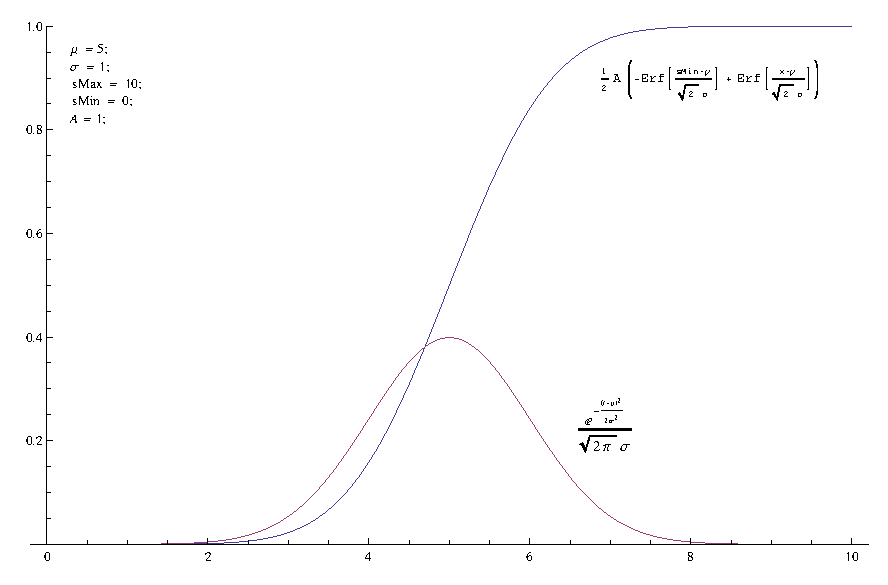
\includegraphics[width=\textwidth]{Chapter2/Figs/errorFunction.eps}
\end{figure}

First, we determine the maximum value taken in the domain. This is simply found by evaluating the function at $\xMax$. It should be noted that --- if the Gaussian distribution is well contained in the source domain --- the maximum value should be equal to the amplitude. For the sake of simplicity, we'll ignore the amplitude of the fitted Gaussian found previously as it is not relevant to the design of the redistribution function. So, to fix the range of the distribution function, we first scale to the range $0:1$ by simply dividing through by the maximum value, and then re-scale to the destination range $\yRange = \yMax - \yMin$ and shift by $\yMin$.


\begin{equation}\label{eq:disFunction}
  dis(x) = \frac{(\yRange) \left(\text{erf}\left(\frac{x-\mu }{\sqrt{2} \sigma }\right)-\text{erf}\left(\frac{\xMin-\mu }{\sqrt{2} \sigma }\right)\right)}{\text{erf}\left(\frac{\xMax-\mu }{\sqrt{2} \sigma }\right)-\text{erf}\left(\frac{\xMin-\mu }{\sqrt{2} \sigma }\right)}+\yMin
\end{equation}


\subsection{Efficiently Implementing the Distribution Function}
Mathematically, the ERF distribution function~(\ref{eq:disFunction}) achieves all the stated objectives. However, on a device we are dealing with discrete numerics and limited processing power, so further analysis is required. Where we're using a discrete domain and range, the distribution is usefully divided into three characteristic behaviours:  where it is constant, where it preserves all the information, and where it selectively preserves information. Looking at the distribution, this divides the source domain into five regions: two where it is effectively constant, two where it is selective, and one region around the mean where it preserves all the information. In order to design an efficient algorithm, it is useful to identify the boundaries of these five regions.

\newcommand{\Keep}{\Omega}
\newcommand{\keep}{\omega}
\newcommand{\eKeep}{\Omega p}
\newcommand{\ekeep}{\omega p}
\newcommand{\Discard}{\Lambda}
\newcommand{\discard}{\lambda}

\subsubsection{The Region Which Discards All Information}
\begin{figure}[h]
\centering
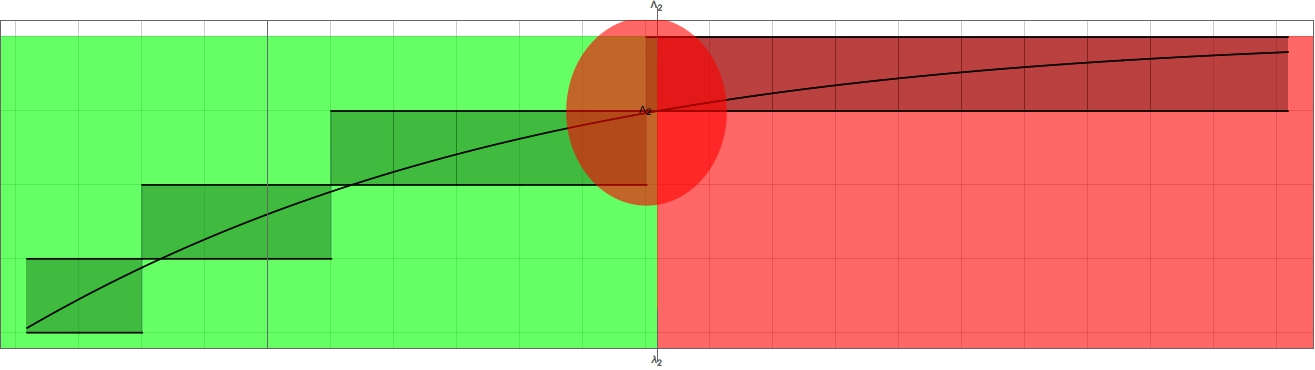
\includegraphics[width=0.7\linewidth]{Chapter2/Figs/EffectivlyConstantRange}
\caption{The region which discards all information beyond $\Discard_2$ is shown above. The shaded grid squares show the value actually taken by the discrete distribution.}
\label{fig:EffectivlyConstantRange}
\end{figure}


First, we need to identify where the distribution is effectively constant. This can be found by solving the following equation in the region and domain $0 \le x \le 1$ and then generalized to the specific discrete numerics:

\begin{equation}\label{eq:0to1}
 \frac{\text{erf}\left(\frac{\mu }{\sqrt{2} \sigma }\right)+\text{erf}\left(\frac{x-\mu }{\sqrt{2} \sigma }\right)}{\text{erf}\left(\frac{\mu }{\sqrt{2} \sigma }\right)-\text{erf}\left(\frac{\mu -1}{\sqrt{2} \sigma }\right)}=\text{dL} \quad \text{where} \quad \text{dL} = \left\{ \frac{1}{\yRange}, 1 - \frac{1}{\yRange} \right\}
\end{equation}


The solution is found for the source domain in the range $0:1$ as:


\begin{equation}\label{eq:LowHigh}
 x = \sqrt{2} \sigma  \text{erf}^{-1}\left((\text{dL}-1) \text{erf}\left(\frac{\mu }{\sqrt{2} \sigma }\right)-\text{dL} \; \text{erf}\left(\frac{\mu -1}{\sqrt{2} \sigma }\right)\right)+\mu
\end{equation}


The boundaries of the regions $x < \Discard_1 $ and $ x > \Discard_2$ for $x \in \{\tMin \cdots \tMax \}$ or $x< \discard_1$  and $ x > \discard_2$ for $x \in \{0 \cdots 1 \}$ can be written using the following helpful constants of the distribution.

\begin{align}\label{eq:DistributionConstants}
\Sigma^- &= \text{erf}\left(\frac{\mu -1}{\sqrt{2} \sigma }\right) &
 \Sigma^+ &= \text{erf}\left(\frac{\mu }{\sqrt{2} \sigma }\right) &
  \text{dL} &= \frac{1}{\yRange} &
  \kappa &= \frac{\yRange}{\tRange} 
\end{align}

\begin{equation}\label{eq:DiscardedRegionBounds}
\begin{aligned}
\discard_1 &= \sigma \sqrt{2} \; \text{erf}^{-1}\left((\text{dL}-1) \Sigma^+-\text{dL} \; \Sigma^-\right)+\mu  &            
\discard_2 &= \sigma \sqrt{2} \; \text{erf}^{-1}\left((\text{dL}-1) \Sigma^- -\text{dL} \; \Sigma^+ \right)+\mu \\
\Discard_1&= \tMin + \tRange \left( \discard_1(\mu,\sigma) \right) & 
\Discard_2 &= \tMin + \tRange \left( \discard_2(\mu,\sigma) \right)
\end{aligned}
\end{equation}

\subsubsection{The Region Which Keeps All Information}
To find the region where all the information in the source domain is preserved, we differentiate the distribution and solve for where the gradient is equal to the destination range over the source range. This corresponds to the point at which a unit change in the source produces a unit change in the destination range:

\begin{equation}\label{eq:Boundaries}
\frac{\sqrt{\frac{2}{\pi }} e^{-\frac{(x-\mu )^2}{2 \sigma ^2}}}{\sigma  \left(\text{erf}\left(\frac{\mu }{\sqrt{2} \sigma }\right)-\text{erf}\left(\frac{\mu -1}{\sqrt{2} \sigma }\right)\right)}=\frac{\yRange}{\tRange}
\end{equation}

Rearranging for $x$, we find:

\begin{equation}\label{eq:PreservedRegion}
 x=\mu \pm \sigma  \sqrt{-2 \log \left(\sigma  \left(\text{erf}\left(\frac{\mu }{\sqrt{2} \sigma }\right)-\text{erf}\left(\frac{\mu -1}{\sqrt{2} \sigma }\right)\right)\right)+2 \log \left(\frac{\tRange}{\yRange}\right)+\log \left(\frac{2}{\pi }\right)}
\end{equation}


The boundaries of the region $\Keep_1 < x < \Keep_2$ for $x \in \{\tMin \cdots \tMax \}$ and $\keep_1 < x < \keep_2$ for $x \in \{0 \cdots 1 \}$ can be written using the following helpful constants of the distribution.

\begin{align}\label{eq:DistributionConstants}
\Sigma^- &= \text{erf}\left(\frac{\mu -1}{\sqrt{2} \sigma }\right) &
 \Sigma^+ &= \text{erf}\left(\frac{\mu }{\sqrt{2} \sigma }\right) &
  \kappa &= \frac{\yRange}{\tRange} 
\end{align}

\begin{equation}
  w(\mu,\sigma)  =  \sigma  \sqrt{ \log \left(\frac{2}{\pi } \right) -2 \log \left(\kappa \sigma  \left(\Sigma^+-\Sigma^-\right)\right) }
\end{equation}

The equations are found in the unit source domain $0:1$. It is a simple matter to scale and shift these values to give the points in a more general source domain.

\begin{equation}\label{eq:PreservedRegionGen}
\begin{aligned}
\keep_1(\mu,\sigma) &=                                    \mu - w(\mu,\sigma) &            \keep_2(\mu,\sigma) &=                                   \mu + w(\mu,\sigma) \\
\Keep_1(\mu,\sigma) &= \tMin + \tRange\left( \mu - w(\mu,\sigma) \right) & \Keep_2(\mu,\sigma) &= \tMin + \tRange \left(\mu +\mu - w(\mu,\sigma)\right)
\end{aligned}
\end{equation}

\begin{figure}[h]
\centering
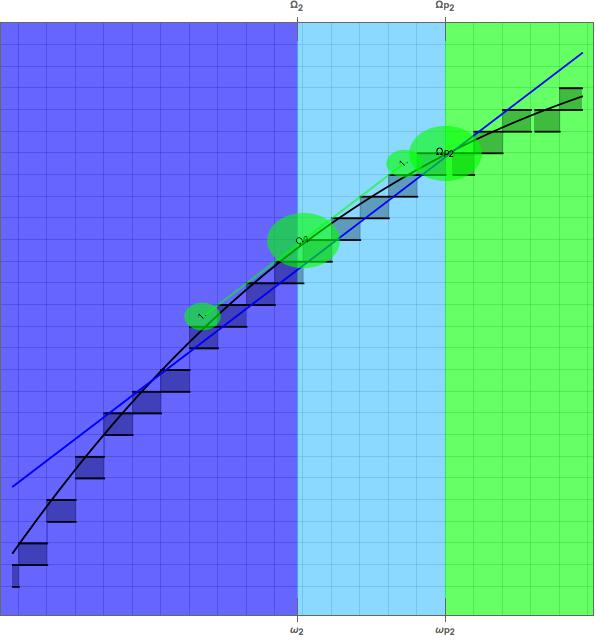
\includegraphics[width=0.7\linewidth]{Chapter2/Figs/ExtensionToLinearRegion}
\caption{The region which preserves all information extends beyond the analytic region due to the rounding involved in the discretization. The shaded grid squares show the value actually taken by the discrete distribution. The cord is the tangent to the distribution curve shifted to the next discrete unit below the curve at $\Keep_2$. The point of intersection is the extended boundary at which the distribution begins to discard information.}
\label{fig:ExtensionToLinearRegion}
\end{figure}

One refinement can be made to these values by recognizing that the discrete distribution extends the effectively linear region past the analytic solution by rounding the values. This can be seen in \ref{fig:ExtensionToLinearRegion}, where the shaded squares are the rounded values. The extended region boundary $\eKeep$ was found by numerically solving 

\begin{equation}
\left\lfloor\text{dis}\left(\Keep _2\right)\right\rfloor+\left(x-\Keep _2\right)=\text{dis}(x)
\end{equation}

In the C++ code, whilst numerical routines were used  MatLab and Mathematica to perform the analysis, the extended region boundary point was found by 'walking' along the distribution from the analytic point $\Keep_2$  until divergence from linear behavior became apparent. This is regarded as a simpler solution, not requiring the use of numerical library routines, and proved to be a quick and elegant solution for the C++ implementation. The extended boundaries $\eKeep_1$ and $\eKeep_2$ are then defined by

\begin{equation}
\begin{aligned}
\left\lceil\text{dis}\left(\Keep _1\right)\right\rceil-\Keep _1 & =\text{dis}\left(\eKeep _1\right)- \eKeep _1 &
\left\lfloor\text{dis}\left(\Keep _2\right)\right\rfloor-\Keep _2 & =\text{dis}\left(\eKeep _2\right)- \eKeep _2 
\end{aligned}
\end{equation}

\subsubsection{The compression ratio}

There is one final value of interest to the development of the algorithm, which is the gradient at the mean. The reason this is of interest is because we're trying to compress the relevant data as much as possible. If the destination region is small (i.e. the destination machine type is smaller than the source type), then the gradient at the mean allows us to assess the fidelity required of the source type. If it weren't for the fact that the source is the result of a rotation transformation, then there would be little purpose in assessing this value. However, it is entirely possible that the lengthening of the axes resulting from the rotation is insignificant for the desired destination type; there's no point preserving information during the rotation which is then discarded by the redistribution. The gradient is given by

\begin{equation}\label{eq:gradient}
\begin{aligned}
\Delta(\mu,\sigma) &= \kappa  \delta(\mu,\sigma)  & \delta(\mu,\sigma)  &= \frac{ \sqrt{2} }{ \sigma \sqrt{\pi }  \left(\Sigma^+-\Sigma^-\right)}
\end{aligned}
\end{equation}

The compression ratio is at most one-to-one, therefore $\kappa <=1$ and the gradient in the unit space must always be greater than one $1 \le \delta(\mu,\sigma)$. so $ \kappa \le \Delta(\mu,\sigma) \le \delta(\mu,\sigma)$.

The required fidelity in the source domain can be found using $ \Delta$ in the sense that the correspondence between one information step in the source must produce a step of $\Delta$ in the destination type. For the algorithm evaluating the maximum gradient $\Delta$ allows us to be sure that  $\Keep$ --- the region on the x axis where all the information is to be preserved --- exists if $\Delta >1$ or tells us that the x axis can be shortened if  $\Delta < 1$. In the algorithm $\Delta$ is used to find an appropriate working data type for the rotated color space and to define the axis scaling for the rotation matrix.


We need to consider the requested compression of information alongside the spread of information caused by the rotation, and the desired focus on the specific region of interest dictated by the statistics. Each axis in the color space is to be represented by a discrete set of numbers. The size of these sets dictates the discretization of the axis, and the ratios between them indicates the spread or compression of the information they contain. We assume that the RGB axes are each discretized to the same extent, each containing $\srcRange$ values. After the application of the un-normalized rotational transformation, the axes contain differing numbers of values given by $\tRange_1 =\srcRange \; \sqrt{3} $, $\tRange_2 = \srcRange \; L_2(\theta) $  and $\tRange_3 = \srcRange \; L_3(\theta)$. These axis lengths preserve all the information contained in the source color space, and so are the maximum length the axis should take. The minumum length the axis may take is where the information is lost evenly throuought the axis, and corresponds to an axis length equal to the destination axis length $\tRange = \dstRange$. 

We can now write an algorithm which determines the necessary scaling for the axes, and whether truncation of the extreme values is significant.
As this will alter $\tRange$ we fix the values of $\kappa$ and $\Delta$ to be those for the working range $\tRange = \mathbf{L}(\theta) \srcRange$  which preserves all information. With this value the constants are
\begin{align}
K & =  \frac{\dstRange}{\srcRange}  &
\kappa(\theta) &=  \frac{K}{\mathbf{L}(\theta)}  & 
\Delta(\mu,\sigma)  &= \frac{K}{\mathbf{L}(\theta)} \delta(\mu,\sigma)  
\end{align}
The length of the axis $\tRange$ after rescaling should be

\begin{equation}\label{eq:CombinedRotationRange}
\begin{aligned}
 \tRange(\theta,\mu,\sigma) &= \min\left\{ \frac{K}{\mathbf{L}(\theta)}   \delta(\mu,\sigma) , 1 \right\} \mathbf{L}(\theta) \srcRange  \\
  & =  \min\left\{K \delta(\mu,\sigma) \right. ,  \left. \mathbf{L}(\theta) \right\}  \srcRange
\end{aligned}
\end{equation}

The scaling $\srcRange$ comes from the source pixel values, the remaining terms translates simply into a rotation matrix scaling

\begin{equation*}
\R[\theta]   =  \min\left\{K \delta(\mu,\sigma) \right. ,  \left. \mathbf{L}(\theta) \right\} \otimes \Scale[\theta] \otimes \fRO \left[   \qRe[ \theta, n ] \right]   \\
\end{equation*}

This satisfies the requirements placed on the gradient $\Delta(\mu,\sigma)>1$ because: if we substitute for $\tRange$ in the definition for the gradient \ref{eq:gradient}

\begin{equation}\label{eq:newGradient}
\begin{aligned}
\Delta(\mu,\sigma) % &= \frac{\dstRange}{\tRange}  \delta(\mu,\sigma)  & \delta(\mu,\sigma)  &= \frac{ \sqrt{2} }{ \sigma \sqrt{\pi }  \left(\Sigma^+-\Sigma^-\right)} \\
% &= \frac{\dstRange}{\min\left\{ \frac{K}{\mathbf{L}(\theta)}   \delta(\mu,\sigma) , 1 \right\} \mathbf{L}(\theta) \srcRange }  \delta(\mu,\sigma) \\
%&= \frac{1}{\min\left\{ \frac{K}{\mathbf{L}(\theta)}   \delta(\mu,\sigma) , 1 \right\} }  \frac{K}{\mathbf{L}(\theta)}   \delta(\mu,\sigma) \\
%&= \begin{cases}
%1 & \frac{K}{\mathbf{L}(\theta)}   \delta(\mu,\sigma) < 1 \\
% \frac{K}{\mathbf{L}(\theta)}   \delta(\mu,\sigma)  & \frac{K}{\mathbf{L}(\theta)}   \delta(\mu,\sigma) > 1 \\
%\end{cases} \\
&= \max\left\{ \frac{K}{\mathbf{L}(\theta)}   \delta(\mu,\sigma) , 1 \right\}
\end{aligned}
\end{equation}
And the compression ratio $\kappa$ is also explicitly restricted to being at most one and now is no longer defined in terms of $\tRange$.
\begin{equation}\label{eq:newCompressionRatio}
\begin{aligned}
\kappa(\theta) % &=  \frac{\dstRange}{\tRange} \\
% &= \frac{\dstRange}{\min\left\{ \frac{K}{\mathbf{L}(\theta)}   \delta(\mu,\sigma) , 1 \right\} \mathbf{L}(\theta) \srcRange }   \\
%&= \frac{1}{\min\left\{ \frac{K}{\mathbf{L}(\theta)}   \delta(\mu,\sigma) , 1 \right\} }  \frac{K}{\mathbf{L}(\theta)}    \\
%&= \begin{cases}
%\frac{1}{\delta(\mu,\sigma)}   & \frac{K}{\mathbf{L}(\theta)}   \delta(\mu,\sigma) < 1 \\
% \frac{K}{\mathbf{L}(\theta)}   & \frac{K}{\mathbf{L}(\theta)}   \delta(\mu,\sigma) > 1 \\
%\end{cases} \\
%&= \max\left\{ \frac{\mathbf{L}(\theta)}{K \delta(\mu,\sigma) }   , 1 \right\} \frac{K}{\mathbf{L}(\theta)}  \\
&= \max\left\{ \frac{1}{\delta(\mu,\sigma) }   , \frac{K}{\mathbf{L}(\theta)} \right\}   
\end{aligned}
\end{equation}



%
%\begin{equation}
%\R[\theta]  = 
%\begin{cases}
% \mathbf{L}(\theta) \otimes \Scale[\theta] \otimes \fRO \left[  \qRe[ \theta, n ] \right]    & \Delta(\mu,\sigma) = 1 \\
%                                        K  \Scale[\theta] \otimes \fRO \left[  \qRe[ \theta, n ] \right]    & \Delta(\mu,\sigma)  = \kappa \\
%        K  \delta(\mu,\sigma)  \Scale[\theta] \otimes \fRO \left[ \qRe[ \theta, n ] \right]    &  \kappa < \Delta(\mu,\sigma) < 1 \\
%\end{cases}
%\end{equation}
%
%\begin{equation}\label{eq:RescaleAxis}
%\R[\theta]  = \min\left\{\Delta(\mu,\sigma), 1 \right\} \mathbf{L}(\theta) \otimes \nS[\theta] \otimes \rS \otimes \fSe (\theta) \otimes\qS[ n ] \otimes \fSs[\theta]  \otimes \fRO \left[ \qRe[ \theta, n ]  \right]  
%\end{equation}
%
%
%\begin{equation}
%\R[\theta]  = 
%\begin{cases}
%   \rS \otimes \fSe (\theta) \otimes\qS[ n ] \otimes \fSs[\theta]  \otimes \fRO \left[ \qRe[ \theta, n ]  \right]   & \Delta(\mu,\sigma) = 1 \\
% \kappa \otimes \mathbf{L}(\theta)  \otimes \nS[\theta] \otimes \rS \otimes \fSe (\theta) \otimes\qS[ n ] \otimes \fSs[\theta]  \otimes \fRO \left[ \qRe[ \theta, n ]  \right]   & \Delta(\mu,\sigma)  = \kappa \\
% \Delta(\mu,\sigma) \mathbf{L}(\theta)  \otimes \nS[\theta] \otimes \rS \otimes \fSe (\theta) \otimes\qS[ n ] \otimes \fSs[\theta]  \otimes \fRO \left[ \qRe[ \theta, n ]  \right]    &  \kappa < \Delta(\mu,\sigma) < 1 \\
%\end{cases}
%\end{equation}
%
%There are several simplifications which can be applied here. Firstly remembering that :
%\begin{align}
%\srcRange &= 2^n &
%\nS[\theta] \otimes \; \mathbf{L}(\theta)  & = 1 \\
%\nS[\theta] \otimes \rS \otimes \fSe (\theta) & = 
%\begin{pmatrix}
% \frac{1}{3}  \\
% \frac{1}{2}\\
% \frac{1}{2} \\
%\end{pmatrix} &
%\qS[ n ] & = 
%\begin{pmatrix}
% 1  \\
% 2^{2-n } \\
% 2^{2-n }  \\
%\end{pmatrix} \\
%\rS \otimes \fSe (\theta) & = 
%\begin{pmatrix}
% \frac{1}{3}  \\
% \frac{1}{2}\\
% \frac{1}{2} \\
%\end{pmatrix}  \otimes \; \mathbf{L}(\theta) &
%\srcRange \; \qS[ n ] & = 
%\begin{pmatrix}
% 2^n  \\
% 4 \\
% 4  \\
%\end{pmatrix} 
%\end{align}
%
%
%\begin{equation}
%\R[\theta]  = 
%\begin{cases}
%\rS \otimes \fSe (\theta) \otimes\qS[ n ] \otimes \fSs[\theta]  \otimes \fRO \left[ \qRe[ \theta, n ]  \right]  & \Delta(\mu,\sigma) = 1 \\
%\nS[\theta] \otimes \rS \otimes \fSe (\theta) \otimes\qS[ n ] \otimes \fSs[\theta]  \otimes \fRO \left[ \qRe[ \theta, n ]  \right]  & \Delta(\mu,\sigma)  = \kappa \\
%\kappa(\theta) \otimes \rS \otimes \fSe (\theta) \otimes\qS[ n ] \otimes \fSs[\theta]  \otimes \fRO \left[ \qRe[ \theta, n ]  \right]  &  \kappa < \Delta(\mu,\sigma) < 1 \\
%\end{cases}
%\end{equation}
%
%\begin{align}\label{eq:RescaleAxis}
%\R[\theta] % & =  \min\left\{ \Delta(\mu,\sigma) , 1\right\} \otimes \srcRange \otimes \; \mathbf{L}(\theta) \otimes \nS[\theta] \otimes \rS \otimes \fSe (\theta) \otimes\qS[ n ] \otimes \fSs[\theta]  \otimes \fRO \left[ \qRe[ \theta, n ]  \right]  \\
%& = \min\left\{ \Delta(\mu,\sigma) , 1\right\}  \otimes \rS \otimes \fSe (\theta) \otimes
%\begin{pmatrix}
%2^n  \\
% 4 \\
%4  \\
%\end{pmatrix}\otimes \fSs[\theta]  \otimes \fRO \left[ \qRe[ \theta, n ]  \right]  \\
%& = \min\left\{ \Delta(\mu,\sigma) , 1\right\}  \otimes \; \mathbf{L}(\theta) \begin{pmatrix}
% \frac{1}{3}  \\
% \frac{1}{2}\\
% \frac{1}{2} \\
%\end{pmatrix} \otimes
%\begin{pmatrix}
%2^n  \\
% 4 \\
%4  \\
%\end{pmatrix}\otimes \fSs[\theta]  \otimes \fRO \left[ \qRe[ \theta, n ]  \right]  \\
%& = \min\left\{ \Delta(\mu,\sigma) , 1\right\}  \otimes \; \mathbf{L}(\theta) \otimes \begin{pmatrix}
% \frac{2^n}{3}  \\
% 2\\
% 2 \\
%\end{pmatrix} \otimes \fSs[\theta]  \otimes \fRO \left[ \qRe[ \theta, n ]  \right]  \\
%\end{align}
%
%We can now re-formulate the transformation matrix in three different ways: pure rotation without rescaling, 
%
%\begin{equation}
%\R[\theta]  = 
%\begin{cases}
%\rS \otimes \fSe (\theta) \otimes\qS[ n ] \otimes \fSs[\theta]  \otimes \fRO \left[ \qRe[ \theta, n ]  \right]  & \Delta(\mu,\sigma) \ge 1\\
%\nS[\theta] \otimes \rS \otimes \fSe (\theta) \otimes\qS[ n ] \otimes \fSs[\theta]  \otimes \fRO \left[ \qRe[ \theta, n ]  \right]  & \begin{array}{c} \delta(\mu,\sigma) = 1 \\
%  \Delta(\mu,\sigma)  = \kappa
% \end{array} \\
%\kappa[\theta] \otimes \rS \otimes \fSe (\theta) \otimes\qS[ n ] \otimes \fSs[\theta]  \otimes \fRO \left[ \qRe[ \theta, n ]  \right]  &  \kappa < \Delta(\mu,\sigma) < 1 \\
%\end{cases}
%\end{equation}
%\begin{align*}
%\nR[\theta] & = \nRa[\theta]+\dnR[\theta] \\
%& = \nS[\theta] \otimes \rS \otimes \fSe (\theta) \otimes\qS[ n ] \otimes \fSs[\theta]  \otimes \fRO \left[ \qRe[ \theta, n ]  + \dqRe[ \theta, n ]  \right]  \\
%& = 
%\begin{pmatrix}
% \frac{1}{3}  \\
% \frac{1}{2}\\
% \frac{1}{2} \\
%\end{pmatrix}
% \otimes
%\begin{pmatrix}
% 1  \\
% 2^{2-n } \\
% 2^{2-n }  \\
%\end{pmatrix}
%\otimes  \fSs(\theta) \otimes \fRO \left[ \qRe[ \theta, n ]  + \dqRe[ \theta, n ]  \right]   \\
%\end{align*}
%
%\begin{equation}\label{eq:Rotation}
% \R_{xyz}(\theta) =
% \begin{pmatrix}
%  \frac{1}{\sqrt{3}} & \frac{1}{\sqrt{3}} & \frac{1}{\sqrt{3}} \\
%  -\sqrt{\frac{2}{3}} \sine{\theta +\Pii{6} } & \sqrt{\frac{2}{3}} \cos (\theta ) & -\sqrt{\frac{2}{3}} \sine{\Pii{6}-\theta } \\
%  -\sqrt{\frac{2}{3}} \cos \left(\theta +\Pii{6}\right) & -\sqrt{\frac{2}{3}} \sin (\theta ) & \sqrt{\frac{2}{3}} \cos \left(\Pii{6}-\theta \right) \\
% \end{pmatrix} \quad \text{for} \quad  
% \begin{array}{c} \Delta(\mu,\sigma) \ge 1 
% \end{array}
%\end{equation}
%
%maximum scaling --- which scales to the destination range
%
%
%\begin{equation}\label{eq:NormRxyz2}
% \overline{\R}_{xyz}(\theta) =
%\kappa
%\bigotimes
%\R_{xyz}(\theta) \quad where \quad
%\begin{array}{c}
%\kappa = \frac{\dstRange }{\srcRange \mathbf{L}(\theta)}
%\end{array} \quad \text{for} \quad    
% \begin{array}{c} \delta(\mu,\sigma) = 1 \\
%  \Delta(\mu,\sigma)  = \kappa
% \end{array}
%\end{equation}
%
% and scaled --- which shortens the axis as much as possible without losing statistically relevant data. 
%
%\begin{equation}\label{eq:CompressedRotation}
% \widetilde{\R}_{xyz}(\theta,\mathbf{\mu},\mathbf{\sigma}) =
%\Delta(\mu,\sigma)
%\bigotimes
%\R_{xyz}(\theta) \quad \text{for} \quad  \kappa < \Delta(\mu,\sigma) < 1
%\end{equation}
%because $\Delta$ is always greater or equal to $\kappa$ these special cases can be combined into a general scaling for each axis
%
%\begin{equation}\label{eq:CombinedRotation}
% \widehat{\R}_{xyz}(\theta,\mu,\sigma) =
%\left(
%\begin{array}{c}
%\min\left\{\Delta(\mu_1,\sigma_1), 1 \right\} \\
%\min\left\{\Delta(\mu_2,\sigma_2), 1 \right\}  \\
%\min\left\{\Delta(\mu_3,\sigma_3), 1 \right\}  \\
%\end{array}
%\right)
%\bigotimes
%\R_{xyz}(\theta) \quad where \quad
%\begin{array}{c}
%\kappa = \frac{\dstRange }{\srcRange \mathbf{L}(\theta)} \\
%\Delta(\mu,\sigma) = \kappa \delta(\mu,\sigma)
%\end{array}
%\end{equation}

\subsubsection{A Piecewise Approximation to the ERF Distribution}
We now have equations which give us the four points in the source domain which mark the boundaries of the five characteristic regions. We can now use them to define a piecewise function which uses the computationally problematic error function based distribution as little as possible

\begin{equation}
pDis(x) = \begin{cases}
\dstMin & x \le \Discard_1 \\
\text{dis}(x) & \Discard_1 < x < \eKeep_1 \\
x - \eKeep_1 + \text{dis}(\eKeep_1) & \eKeep_1 \le x \le \eKeep_2  \\
\text{dis}(x) + \eKeep_2 - \eKeep_1 - \text{dis}(\eKeep_2) + \text{dis}(\eKeep_1)  & \eKeep_2 < x < \Discard_2  \\
\text{dis}(\Discard_2) + \eKeep_2 - \eKeep_1 - \text{dis}(\eKeep_2) + \text{dis}(\eKeep_1) & x \ge \Discard_2 \\
\end{cases}
\end{equation}

All three distribution techniques ( \ref{sec:Partition} , \ref{sec:Linear} , \ref{sec:ERF} ) described earlier are special cases of this distribution. When the distribution has a very large variance the piecewise distribution can be simplified as a linear distribution fig\ref{fig:useLinear}. When the distribution has a very small variance a partitioning is more appropriate fig \ref{fig:usePartitioning}. The most interesting distributions, however, are the ones which require the use of the piecewise distribution fig \ref{fig:usePiecewiseERF}. 

\begin{figure}[h]
\centering
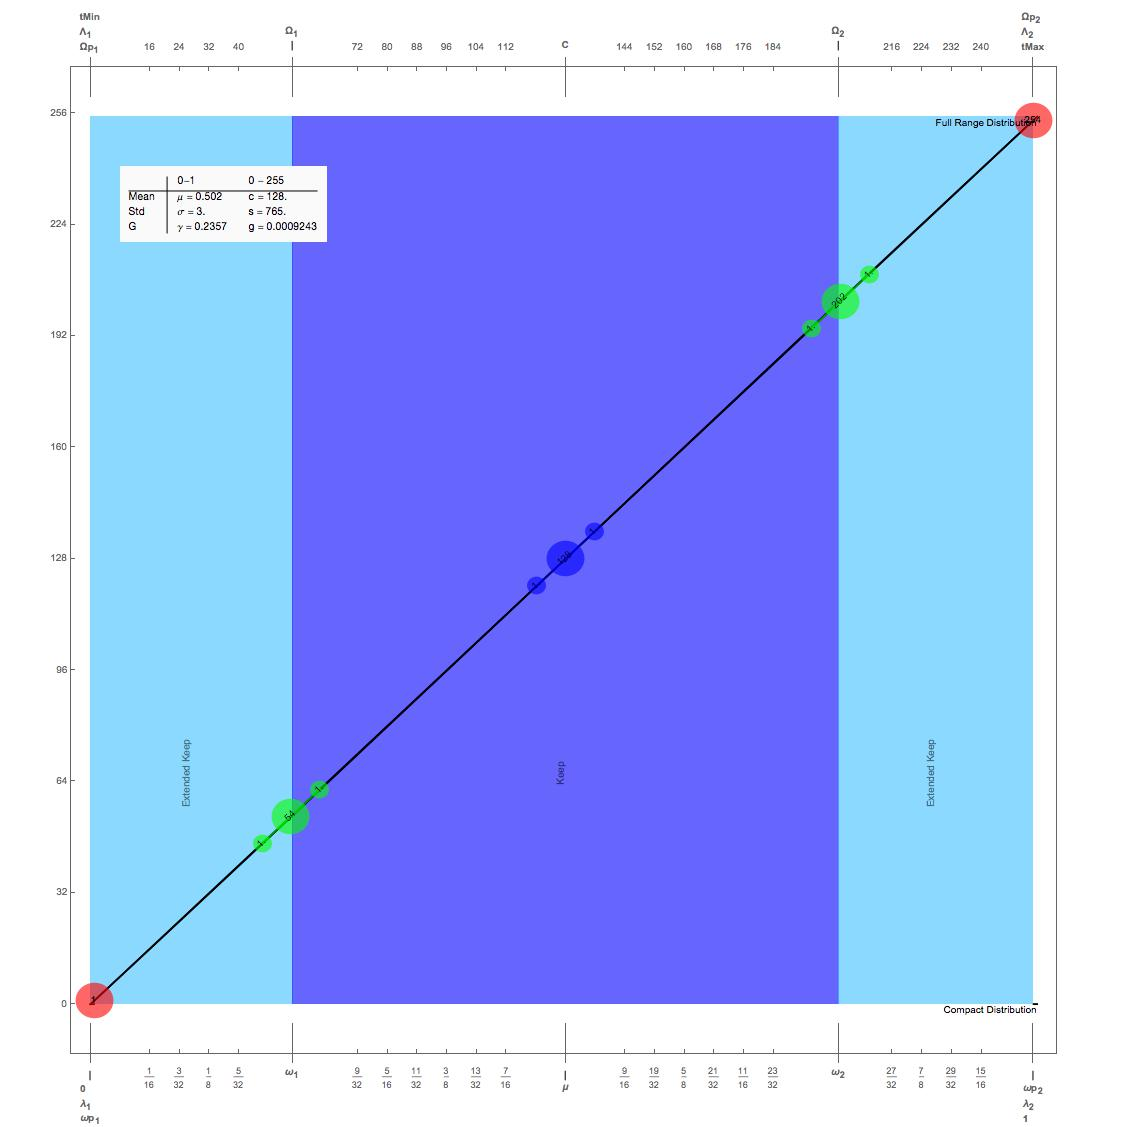
\includegraphics[width=1\linewidth]{Chapter2/Figs/useLinear}
\caption{Here the code will decide to use a linear redistribution.}
\label{fig:useLinear}
\end{figure}

\begin{figure}[h]
\centering
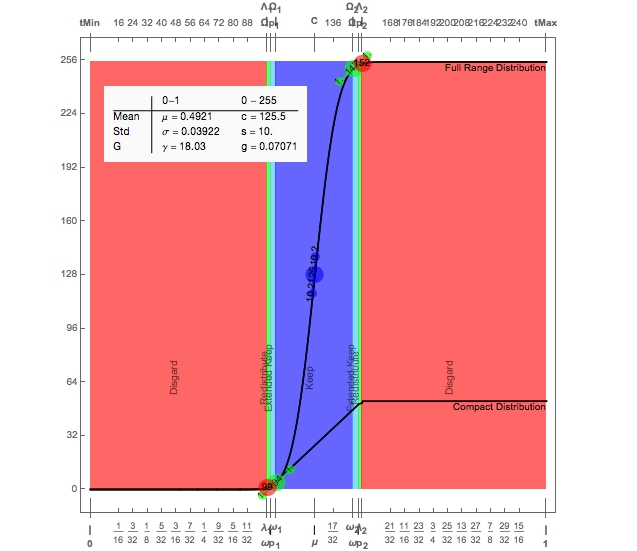
\includegraphics[width=1\linewidth]{Chapter2/Figs/usePartitioning}
\caption{With these values the code will likely decide to use partitioning if the tolerance $\tau_{\text{partitioning}}$is greater than $\Discard_2-\eKeep_2$.}
\label{fig:usePartitioning}
\end{figure}

\begin{figure}[h]
\centering
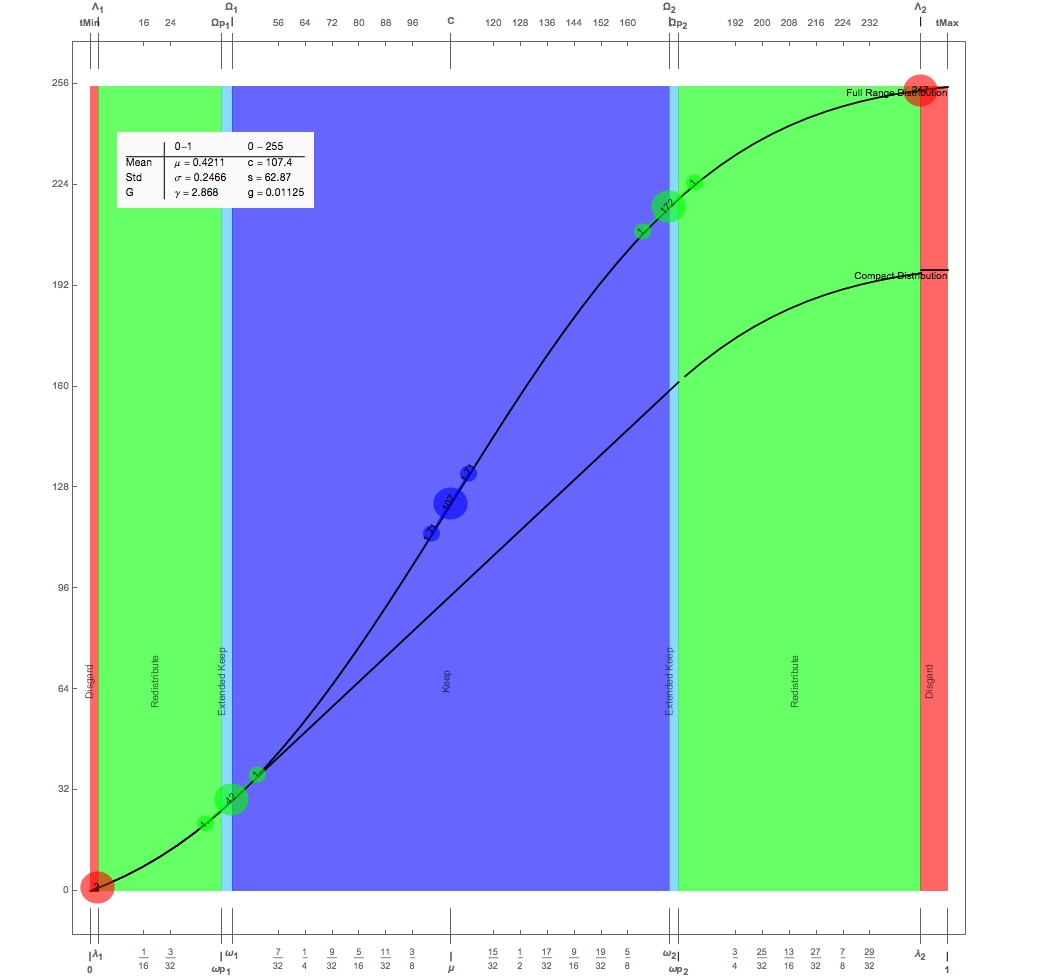
\includegraphics[width=1\linewidth]{Chapter2/Figs/usePiecewiseERF}
\caption{With these values the code will decide to use a piecewise ERF based distribution (Labeled Compact Distribution in the figure).}
\label{fig:usePiecewiseERF}
\end{figure}


\section{The Skin Color Space Algorithm}
\newcommand{\uSTD}[1]{\sigma_#1}
\newcommand{\STD}[1]{\text{s}_#1}
\newcommand{\uMean}[1]{\mu_#1}
\newcommand{\mean}[1]{\text{c}_#1}

Now that all of the values necessary to preserve the skin information have been obtained, we can use them to build a color space transformation algorithm which can make intelligent decisions about the numerical precision for the intermediate and final variables, as well as determining the most efficient transformation methods. The algorithm described herein will take values of $\theta$, the rotation about the luminosity axis, the standard deviations $ \uSTD{a}$,$ \uSTD{b}$ and mean values $ \uMean{a}$,$ \uMean{b}$ for the two chromatic axes in the unit range  and will automatically decide upon the necessary intermediate working data types and the most efficient redistribution methods.

Previously, we found a rotational transformation which allows a working type $\tRange$ to be chosen such that $\tRange \le 2 \srcRange$. If we were to keep the same data type for the color space $\dstRange$ as is used for the RGB values $\srcRange$, then the axes would have to be rescaled with the accompanying loss of information. Given that we have values which allow us to assess where all the relevant information lies, a more sophisticated approach is possible. For a chromatic axis --- which, after rotation, has a length $L(\theta)$ --- we can determine the positions on that axis at which the information is considered irrelevant using Equation~(\ref{eq:LowHigh}) and the positions where the information is all considered relevant. If the gradient $ \Delta$ \ref{eq:gradient} is less than 1, then the distribution loses information at all points on the axis and the axis can be shortened without loss of relevant information. The only further consideration is to ensure that the values outside that range are prevented from causing errors associated with overflow. To exclude this possibility, a conditional statement can be used which checks the bounds as stated, assigning an appropriate value as necessary. The alternative is to use an intermediate value with a higher bit depth, and then to recast into the destination data type in such a way that overflow and underflow are handled appropriately. The OpenCV library provides a casting method --- "saturateCast" --- which serves this purpose.



%You know those blue/black people? Melanin may not be expressed in the fingernails!

%\subsection{Pigment vs. Blood}\label{sec:PigmentVs.Blood}

%\subsection{Blood Flow}\label{sec:BloodFlow}

%\subsection{Amplify the Effect}\label{sec:AmplifyTheEffect}

